\documentclass[11pt]{article}
\usepackage{titling}
\usepackage{multicol}
\usepackage{media9}
\usepackage[english]{babel}
\usepackage[margin=0.6in]{geometry} % Page Dimension
\setlength{\parindent}{0pt}

%%%%%%%%%%%%%%%%%%%%%%%%%%%%%%%%%%%%%%%%%%
%                PACKAGES                %  
%%%%%%%%%%%%%%%%%%%%%%%%%%%%%%%%%%%%%%%%%%

% Styling Choices
\setlength{\parskip}{\baselineskip}%
\renewcommand{\baselinestretch}{1.2}

% Math
\usepackage{amsmath, amsthm, amssymb}
\usepackage[inline]{asymptote}
\usepackage{enumitem,xcolor}
\usepackage{cancel}
\usepackage{gensymb}

% Blind Footnote
\newcommand\blfootnote[1]{%
  \makeatletter{\footnotetext{#1}\makeatother}
}

% Fancy Header
\usepackage{fancyhdr}
\pagestyle{fancy}
\lhead{Kalda Electricity and Magnetism}
\rhead{\thepage}

% Coloured Boxes
\usepackage{xcolor}
\definecolor{border}{HTML}{dd1d1d} % 004D4D
\definecolor{hard}{HTML}{ffccb3}
\definecolor{easy}{HTML}{b3e6b3}
\definecolor{normal}{HTML}{f2f2f2}
\definecolor{ans}{HTML}{00b9f2}
\usepackage{empheq}
\newcommand*\widefbox[1]{\fbox{\hspace{1em}#1\hspace{1em}}}
\definecolor{claim}{HTML}{BA0030}
\newcommand\boldclaim[1]{\textcolor{claim}{\textbf{#1}}}

% Allows for hyperlinking
\usepackage{hyperref}
\hypersetup{
    colorlinks=true,
    urlcolor=magenta,
    linkcolor=ans,
}

% Syntax: \colorboxed[<color model>]{<color specification>}{<math formula>}
\newcommand*{\colorboxed}{}
\def\colorboxed#1#{%
  \colorboxedAux{#1}%
}
\newcommand*{\colorboxedAux}[3]{%
  % #1: optional argument for color model
  % #2: color specification
  % #3: formula
  \begingroup
    \colorlet{cb@saved}{.}%
    \color#1{#2}%
    \boxed{%
      \color{cb@saved}%
      #3%
    }%
  \endgroup
}

% Setup Gray Solution Boxes
\usepackage[breakable,many]{tcolorbox}
\newtcolorbox[auto counter]{solution}[1]{
    enhanced, breakable,
    arc=0pt,
    % colback=default, % Background color
    colframe=white, % Border Color
    coltitle=black, % Title Color
    fonttitle=\bfseries,
    title=\fcolorbox{border}{#1}{\textcolor{border}{pr} \bfseries \textcolor{border}{\thetcbcounter}.},
    attach title to upper,
    after title={\ },
    segmentation style={dashed, gray},
}

% Title and front page
\title{Translated Problems in Electricity and Magnetism Handout by Valter Kiisk}
% Author
\author{\textsc{Daniel Yang, Kushal Thaman}}

\begin{document}
\begin{titlepage}
    \begin{center}
        \vspace*{1cm}
 
        \Huge
        \textbf{Translation of Problems in “Elektri Ja Magnetismi Ülesandeid”}
 
        \vspace{0.5cm}
        \LARGE
        Edition 2.0.0
        
        \vspace{1cm}
        Daniel Yang, Kushal Thaman

\begin{center} % might change this image later
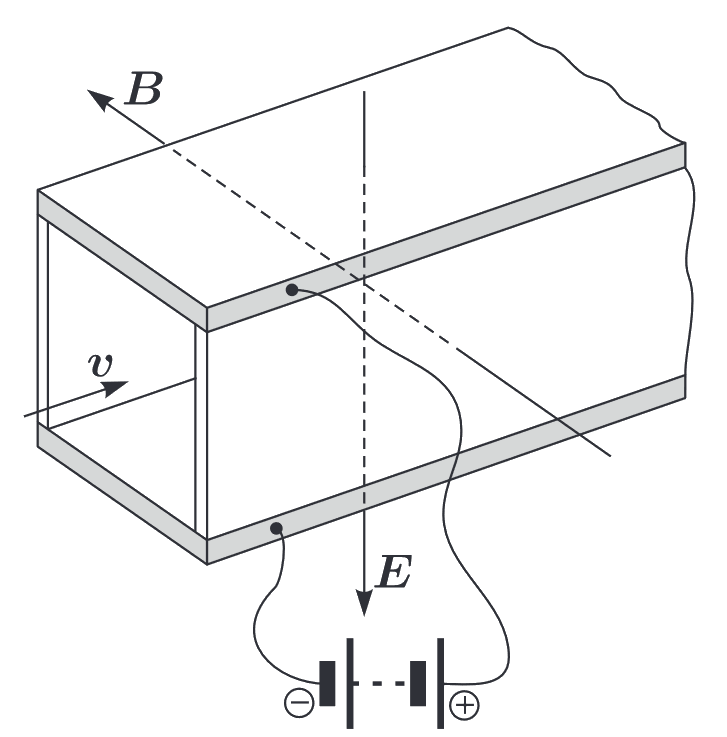
\includegraphics[scale=0.47]{Title.png}
\end{center}
        \vfill
        \Large
        Edited by: Ashmit Dutta, QiLin Xue
        
        \Large
        Updated
        \today
 
    \end{center}
\end{titlepage}
\newpage
%%%%%%%%%%%
% Preface %
%%%%%%%%%%%
\section*{Preface}
\vspace{-5mm}
\indent Jaan Kalda's \href{https://www.ioc.ee/~kalda/ipho/}{handouts} are beloved by physics students both in for a quick challenge, to students preparing for international Olympiads. The current \href{https://www.ioc.ee/~kalda/ipho/Elekter.pdf}{electricity and magnetism} handout (written by Valter Kiisk, ver 2.0) is, unfortunately for people not fluent in Estonian, fully in Estonian. Here, we have attempted to translate all 175 problems in the handout.

\subsection*{Contact Us}
\vspace{-5mm}
Because none of the authors of this document actually know Estonian, we used a combination of Google Translate and observing similarities between the handout and other English-language documents. As a result, some of the translations here are likely wrong or a misinterpretation of the original text. If you do find any mistakes, or know the source of a specific problem, then please contact us at \href{mailto:hello@physoly.tech}{hello@physoly.tech}. The most current and updated version of this document can be found on our website \href{https://physoly.tech/}{physoly.tech}.

Additionally, as we are also high school students and do not have the time to translate 33 pages of hardcore Estonian physics terminology, this document will only contain the problems provided in the handout, and will thus require a significant amount of background knowledge to understand and complete. Since the handout didn't have answers for all the problems, the answers section is incomplete; however, we will update it as the problems are solved (and hopefully we can release a solutions document sometime in the future).

Please feel free to contact us at the same email if you are confused on a question. Chances are that many others will have the same question as you.

\newpage
\section{DC Circuits}
\hypertarget{P1}{}
\begin{solution}{normal} % 1
For an overcurrent protection, there are two fuses connected in parallel: fuse $A$ has resistance $R_A= 1\;\Omega$ and maximal current (by which it melts) $I_{A_\text{max}}= 1 \;\text{A}$; fuse $B$ has resistance $R_B= 2\;\Omega$ and maximal current (by which it melts) $I_{B_\text{max}}= 1.2\;\text{A}$. What is the maximal total current for such a system of fuses? What is the total current when the fuse $B$ is substituted with a fuse $C$ which has $R_C= 2\;\Omega$ and $I_{C_\text{max}}= 1.7\;\text{A}$? (Kalda Circuits P32)
\end{solution}

\hypertarget{P2}{}
\begin{solution}{normal} % 2
The measuring range of a microammeter is $100\;\mu\text{A}$. At this current, there is a voltage drop of $0.1\;\text{V}$ across the terminals of the ammeter. How should a resistor be connected and how large should its resistance be to mimic a) a voltmeter with a measuring range of $100\;\text{V}$ and b) an ammeter with a measuring range of $10\;\text{A}$?
\end{solution}

\hypertarget{P3}{}
\begin{solution}{normal} % 3
A light bulb with power $100\;\text{W}$ is designed for an input voltage of $110\;\text{V}$. What is the resistance of the resistor that should be connected in series to the light bulb such that it has the same brightness with an input voltage of $127\;\text{V}$?
\end{solution}

\hypertarget{P4}{}
\begin{solution}{normal} % 4
Eight identical fluorescent lamps are connected to a constant voltage source as shown in the figure below. There is a resistor in series with the voltage source with resistance equal to that of a single lamp. Does the power emitted by the lamps increase or decrease if one of the lamps burn out? If multiple lamps burn out? Ignore the temperature dependence of the resistance of the lamps. (Similar to Kalda Circuits P41)
\begin{center}
    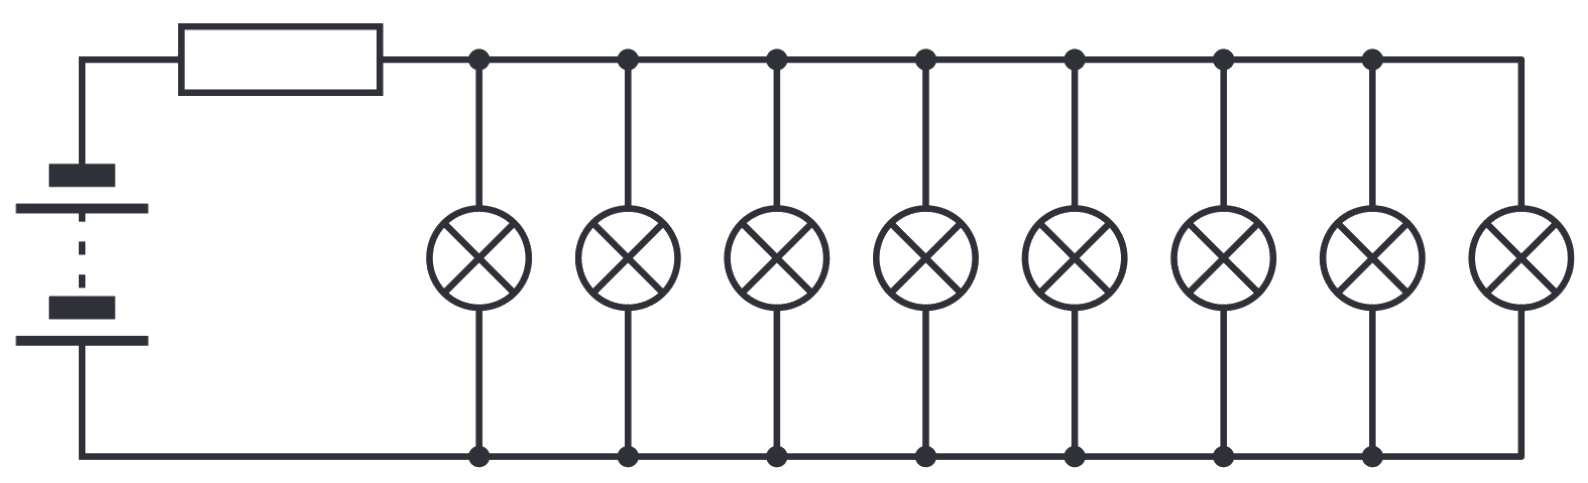
\includegraphics[width=0.55\textwidth]{S1 Figures/S1-4.png}
\end{center}
\end{solution}

\hypertarget{P5}{}
\begin{solution}{normal} % 5
A piece of wire with total resistance $R_0$ is shaped into a closed ring, as shown in the figure below. Two contacts are soldered onto the side of this ring. Determine the resistance between the two contacts if $\alpha=120\degree$.
\begin{center}
    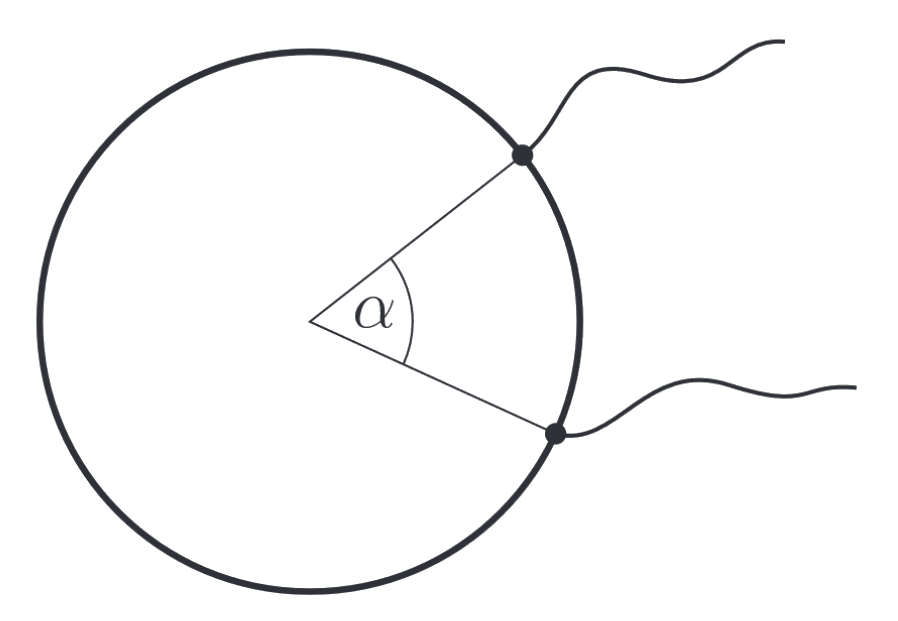
\includegraphics[width=0.31\textwidth]{S1 Figures/S1-5.png}
\end{center}
\end{solution}

\hypertarget{P6}{}
\begin{solution}{normal} % 6 ? kinda unsure about translation
To determine the resistivity of ocean water, a marine scientist immerses a cable of length $50\;\text{mm}$ in the water. The cable consists of two concentric cylindrical electrodes with inner diameter $40\;\text{mm}$ and outer diameter $45\;\text{mm}$. If the resistance between the electrodes is $9\;\Omega$, determine the resistivity of the water.
\end{solution}

\hypertarget{P7}{}
\begin{solution}{normal} % 7
A uniform wire of cross-sectional area $A_0=1\;\text{mm}^2$ had a millimetre scale marked on it: an array of streaks with inter-streak distance $a_0=1\;\text{mm}$ covered the entire length of the wire. The wire was stretched in a non-uniform way, so that the inter-streak distance $a$ is now a function of the distance $l$ from one end of the wire (as measured after the stretching), see figure.The new length of the wire is $L=4\;\text{m}$. Using the graph, determine the electrical resistance $R$ of the stretched wire assuming that the resistivity of the wire material is $\rho=1.0\times10^{-6}\;\Omega\;\text{m}$. During the stretching, the density of the wire material remains constant. \textit{Note:} If a problem contains graphical data, the solution usually comes down to area of the graph, its slope, or intersections in the graph. (Kalda Circuits P1)
\begin{center}
    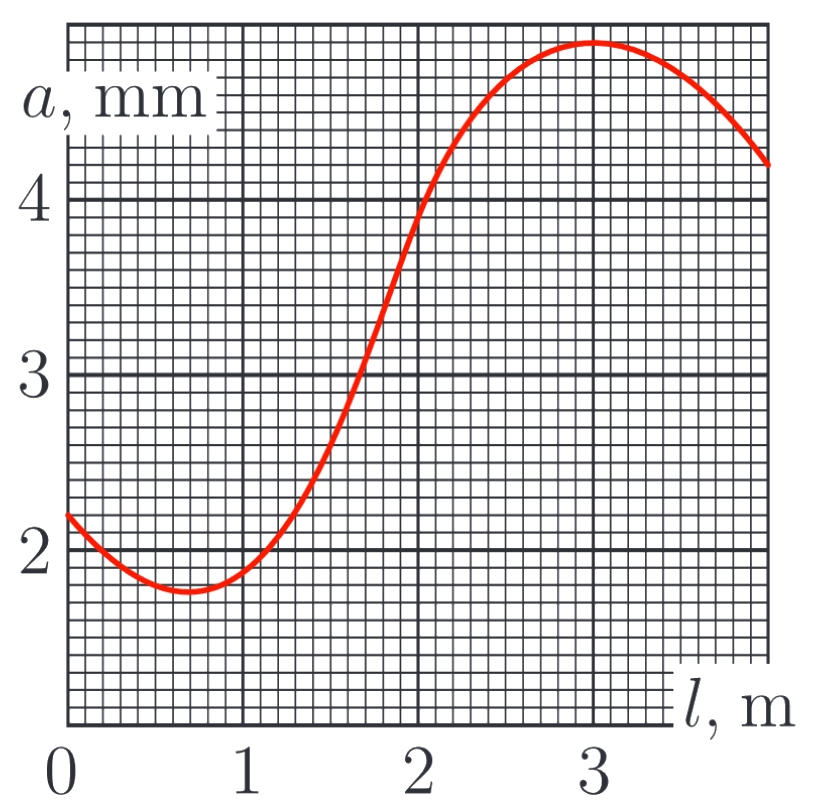
\includegraphics[width=0.48\textwidth]{S1 Figures/S1-7.png}
\end{center}
\end{solution}

\hypertarget{P8}{}
\begin{solution}{normal} % 8
The figure below shows part of a larger circuit. Four identical ammeters, each with an internal resistance of $100\;\Omega$, are connected to the circuit. The readings on the first and second ammeters are $3\;\text{mA}$ and $\text{5mA}$, respectively. Determine the resistance of resistor $R$.
\begin{center}
    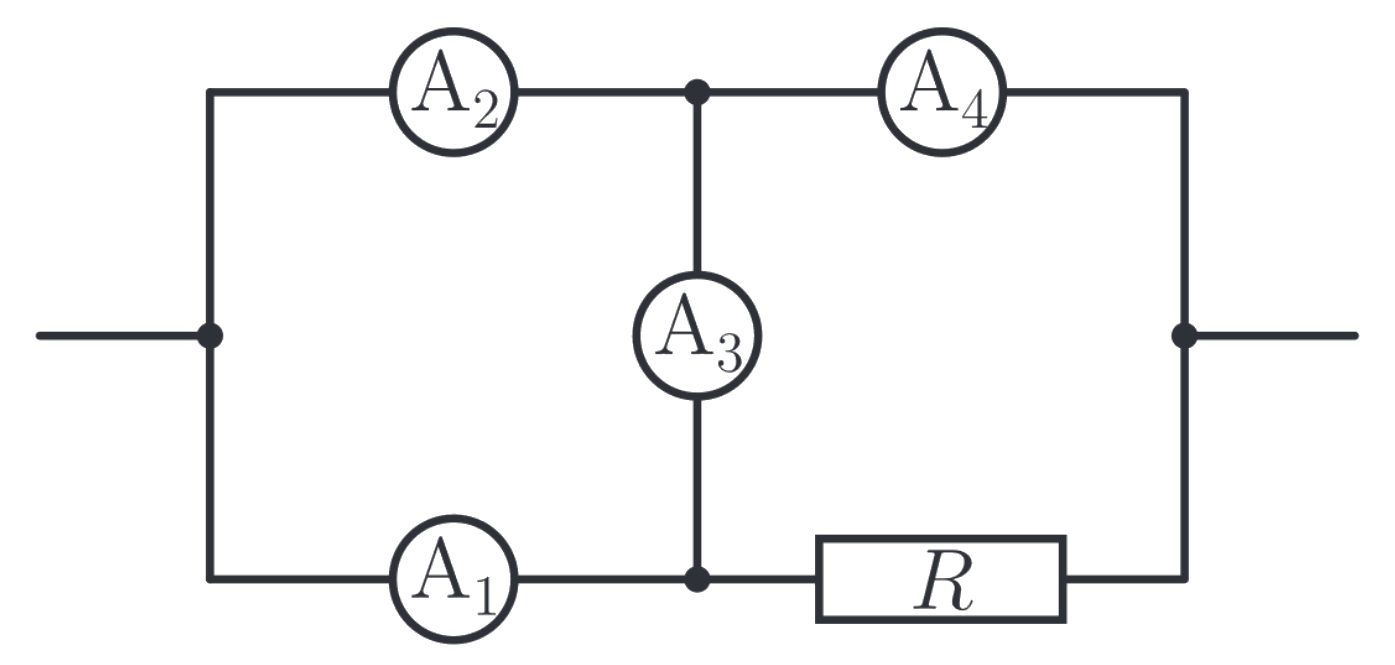
\includegraphics[width=0.55\textwidth]{S1 Figures/S1-8.png}
\end{center}
\end{solution}

\hypertarget{P9}{}
\begin{solution}{normal} % 9
The circuit in the figure below consists of three identical voltmeters and three identical resistors. If the reading on the first voltmeter is $19\;\text{V}$ and the reading on the third voltmeter is $9\;\text{V}$, find the reading on the second voltmeter. (Similar to Kalda Circuits P39)
\begin{center}
    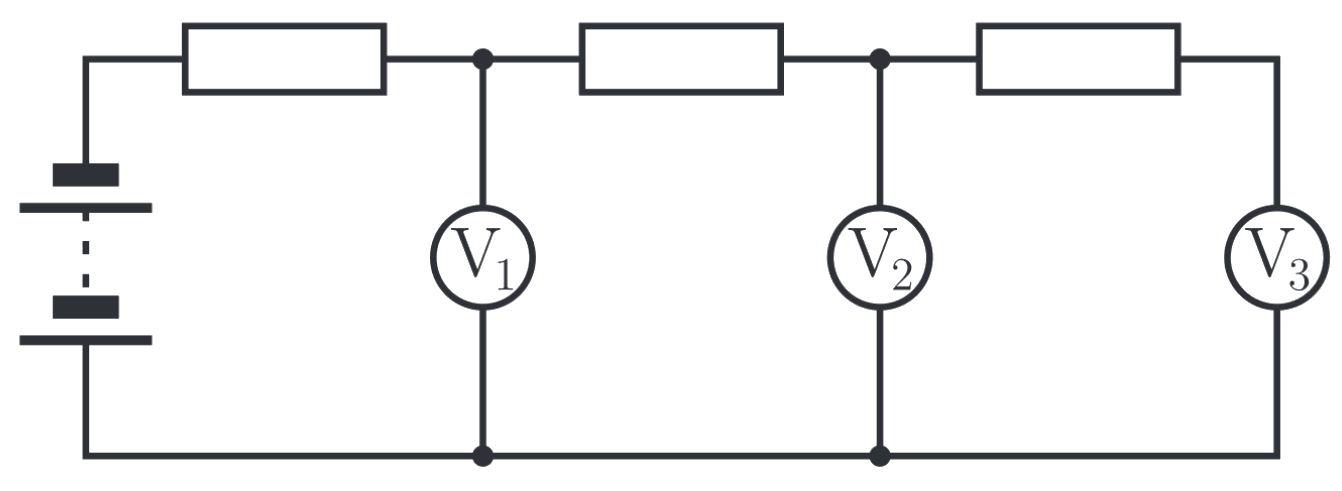
\includegraphics[width=0.65\textwidth]{S1 Figures/S1-9.png}
\end{center}
\end{solution}

\hypertarget{P10}{}
\begin{solution}{normal} % 10
Determine the resistance of the circuit shown below using both the potential and current methods. \textit{Note:} To simplify the statements, you may consider a current of $1\;\text{A}$ passing through the circuit or that the output terminals are connected to a $1\;\text{V}$ voltage source. In the first case, the voltage drop between the ends of the circuit is numerically equal to the effective resistance, and in the second case, the current through the circuit is numerically equal to the inverse of the resistance. (Similar to Kalda Circuits P1)
\begin{center}
    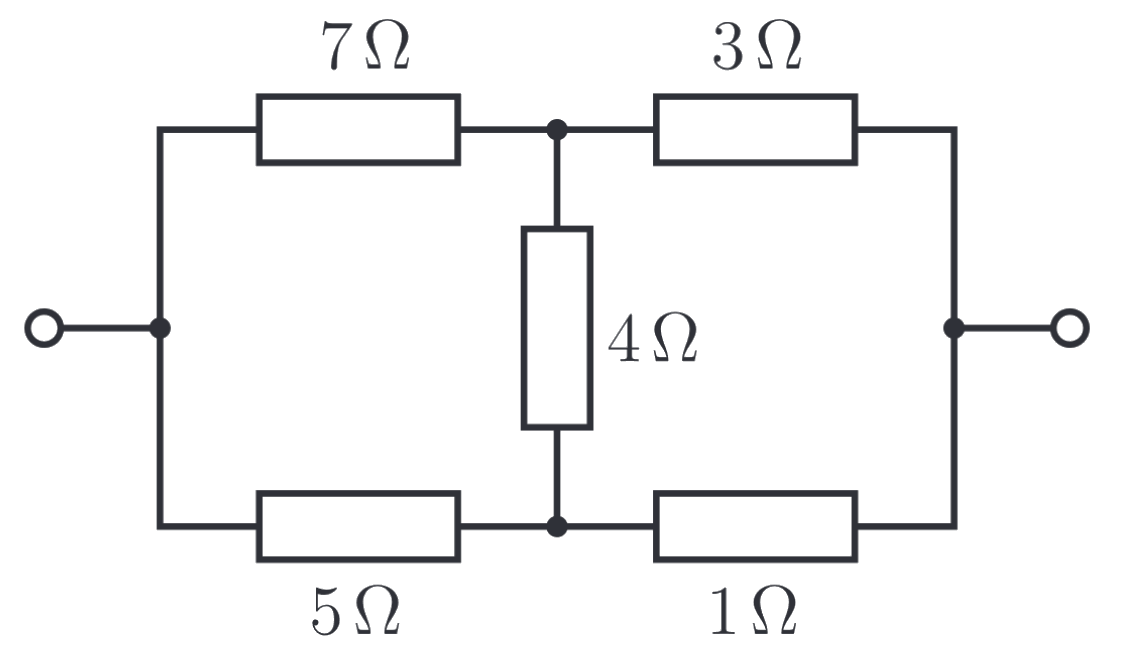
\includegraphics[width=0.55\textwidth]{S1 Figures/S1-10.png}
\end{center}
\end{solution}

\hypertarget{P11}{}
\begin{solution}{normal} % 11
In the figure, $R_1/R_2=4$. If we add a lamp as shown in the figure below, the current through $R_1$ will increase by $\Delta I= 0.1\;\text{A}$. Determine the current through the lamp. (Kalda Circuits P2)
\begin{center}
    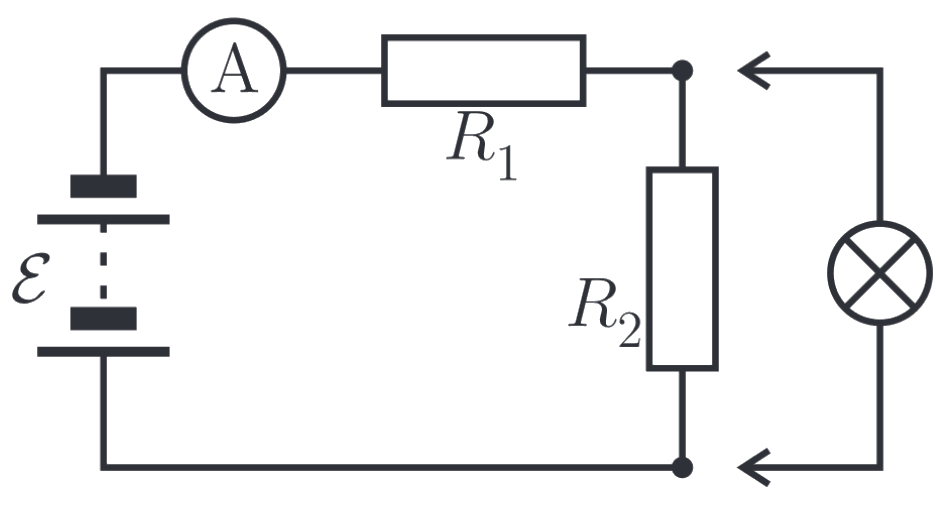
\includegraphics[width=0.5\textwidth]{S1 Figures/S1-11.png}
\end{center}
\end{solution}

\hypertarget{P12}{}
\begin{solution}{normal} % 12
Determine the current through resistor $R_3$ in the circuit shown below.
\begin{center}
    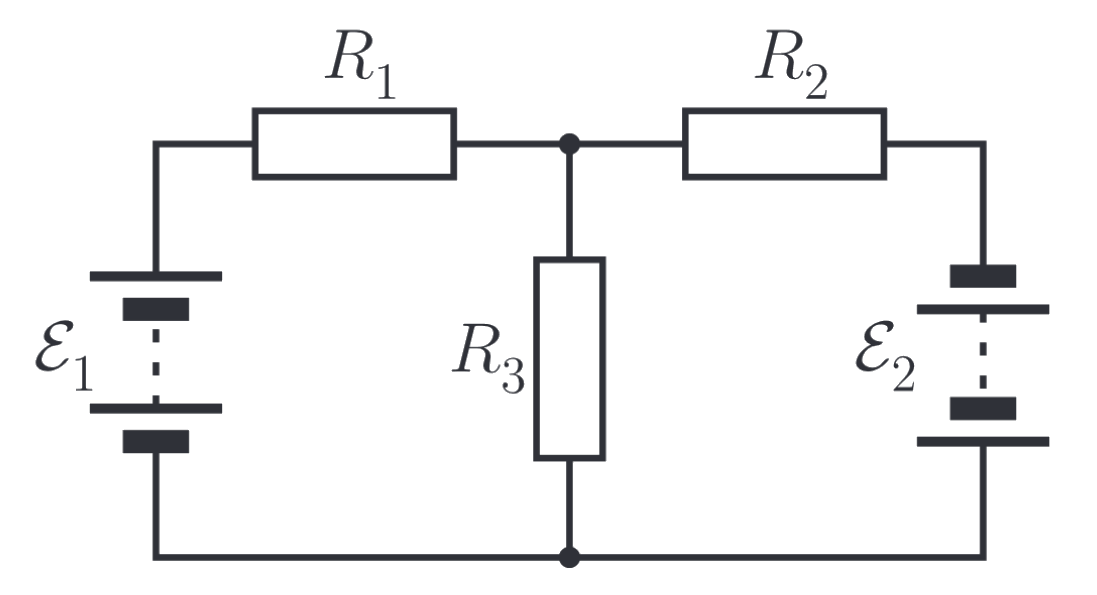
\includegraphics[width=0.6\textwidth]{S1 Figures/S1-12.png}
\end{center}
\end{solution}

\hypertarget{P13}{}
\begin{solution}{normal} % 13
Determine the current through the $8\;\Omega$ resistor. (Similar to Kalda Circuits P12)
\begin{center}
    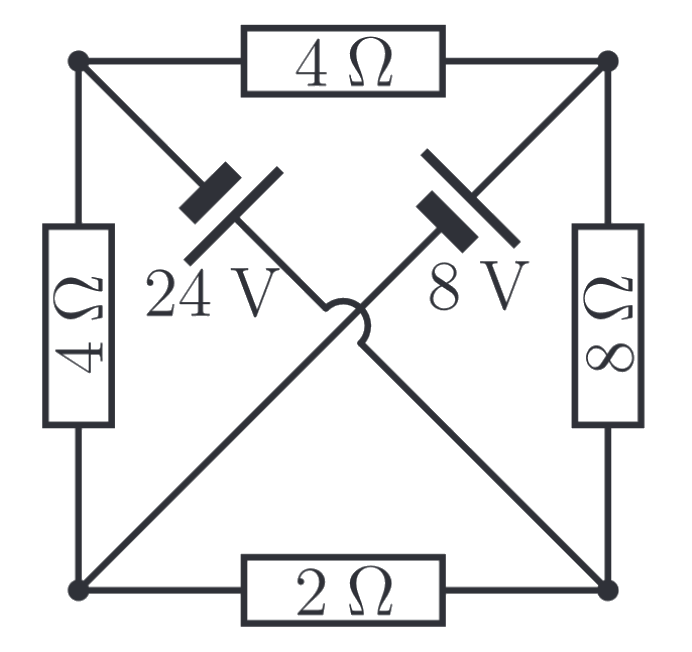
\includegraphics[width=0.38\textwidth]{S1 Figures/S1-13.png}
\end{center}
\end{solution}

\hypertarget{P14}{}
\begin{solution}{normal} % 14
Determine the currents through the batteries. (Kalda Circuits P9)
\begin{center}
    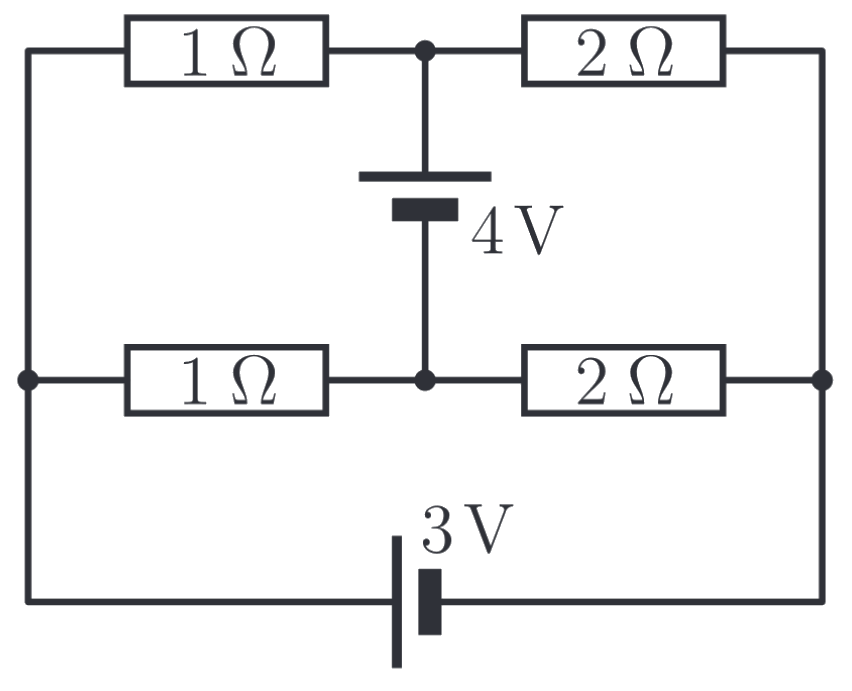
\includegraphics[width=0.45\textwidth]{S1 Figures/S1-14.png}
\end{center}
\end{solution}

\hypertarget{P15}{}
\begin{solution}{normal} % 15
Determine the resistance of the circuit shown below.
\begin{center}
    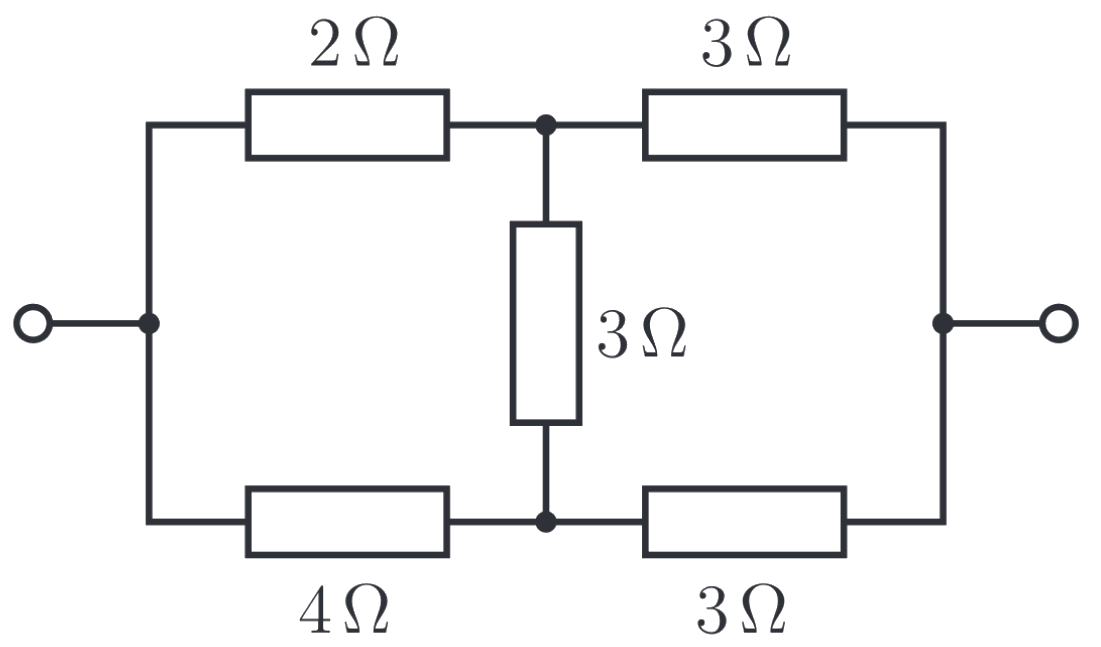
\includegraphics[width=0.6\textwidth]{S1 Figures/S1-15.png}
\end{center}
\end{solution}

\hypertarget{P16}{}
\begin{solution}{normal} % 16 ? kinda unsure about translation
To make Christmas decorations, Juku took 10 identical light bulbs (with a rated voltage of $3\;\text{V}$ and a rated power of $0.6\;\text{W}$), and a rectifier with terminal voltage of $5\;\text{V}$. Based on this, he designed the circuit shown below. He then calculated the necessary value of $R$ such that the voltage across the bulbs is the same as their rated voltage. However, when the rectifier was switched on, the bulbs were still dimmer than expected. Further testing showed that the terminal voltage of the rectifier had dropped to $4\;\text{V}$ and that the voltage across the bulbs had dropped to $2.4\;\text{V}$. How large should $R$ be to light the bulbs to their normal brightness?
\begin{center}
    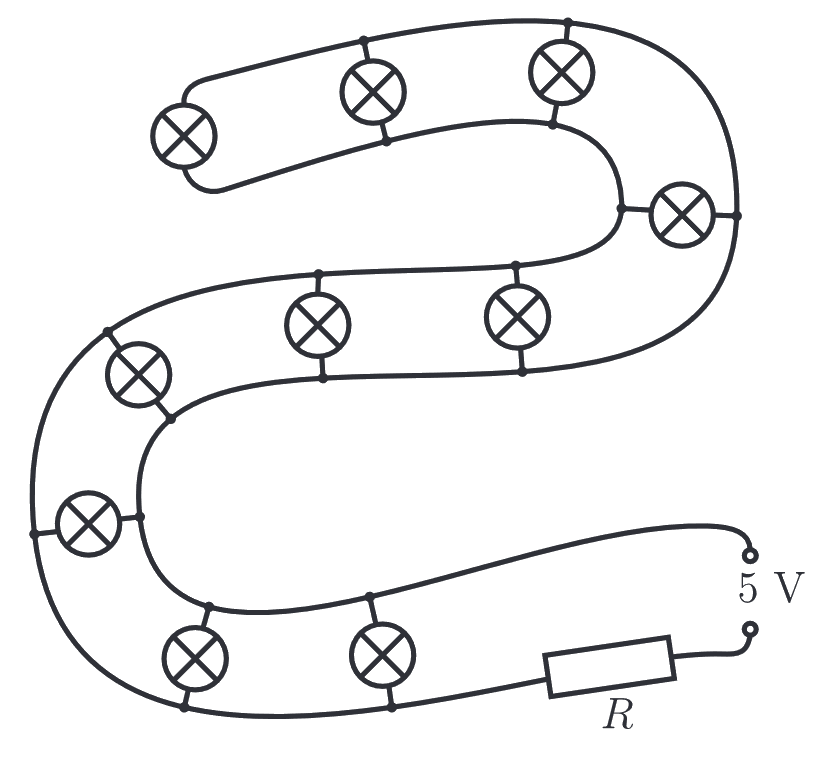
\includegraphics[width=0.7\textwidth]{S1 Figures/S1-16.png}
\end{center}
\end{solution}

\hypertarget{P17}{}
\begin{solution}{normal} % 17
The maximum current ($\mathcal{E}/r$) is obtained from the voltage source if the resistance of the external circuit is zero (i.e. the terminals are short-circuited). However, in this case, the electrical power consumed in the external circuit is also zero. Show that the maximum net power is obtained from a voltage source if the external circuit resistance is equal to the internal resistance of the source.
\end{solution}

\hypertarget{P18}{}
\begin{solution}{normal} % 18
What is the maximum power that can be drawn from the output terminals of the circuits shown below Problem 19?
\end{solution}

\hypertarget{P19}{}
\begin{solution}{normal} % 19
Solve the previous problem using equivalent circuits.
\begin{center}
    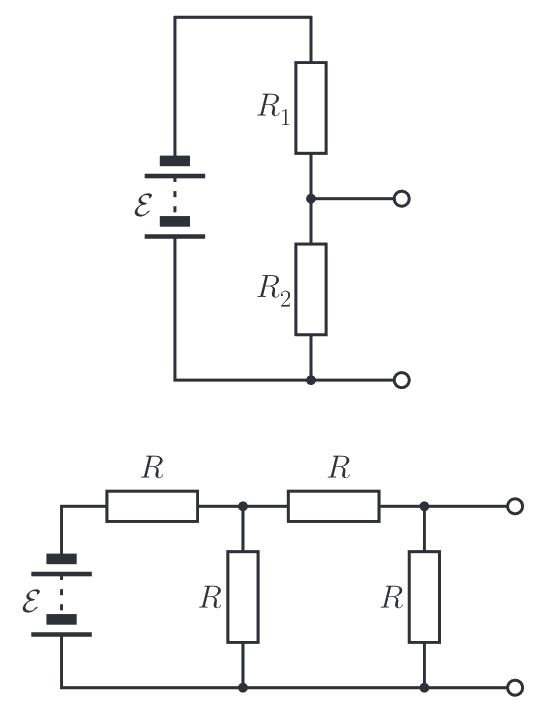
\includegraphics[width=0.42\textwidth]{S1 Figures/S1-18-19.png}
\end{center}
\end{solution}

\hypertarget{P20}{}
\begin{solution}{normal} % 20
In the circuit shown below, determine the voltage at the output terminals and the current through a $10\;\text{k}\Omega$ resistor if the switch $K$ is a) open; b) closed.
\begin{center}
    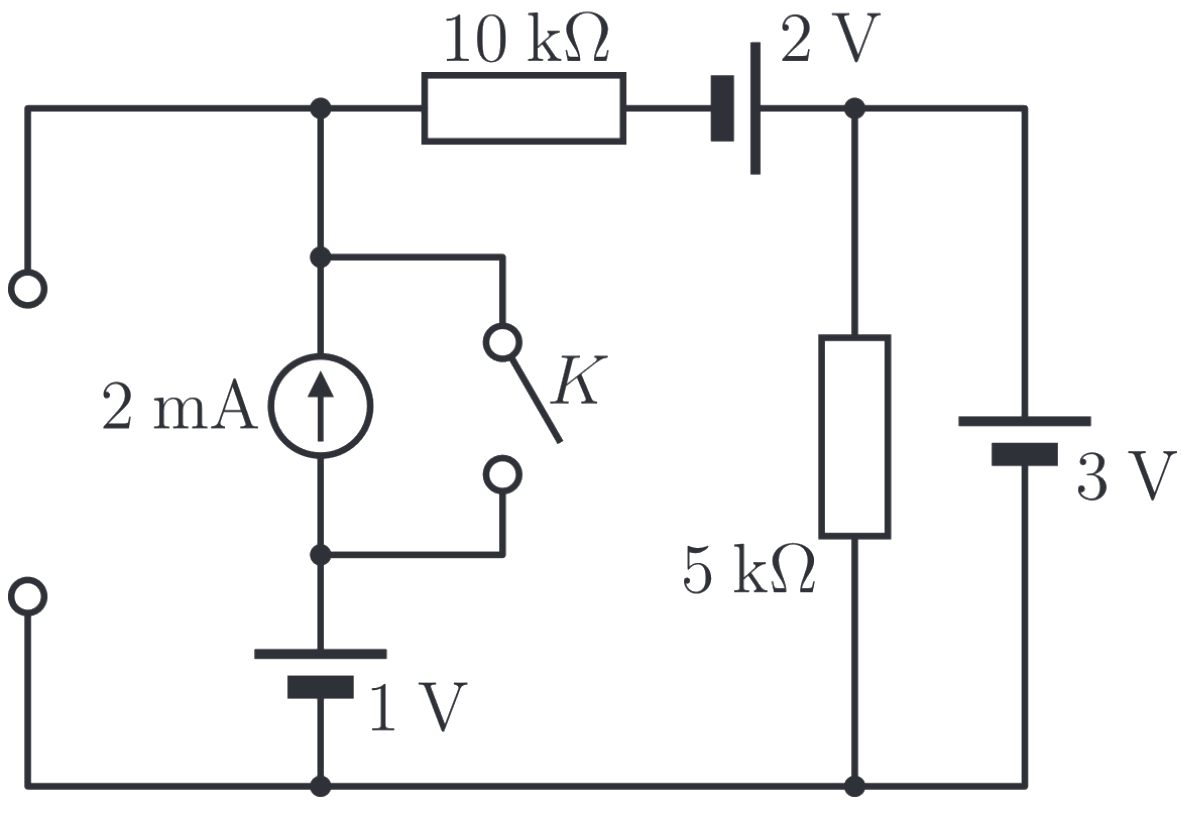
\includegraphics[width=0.45\textwidth]{S1 Figures/S1-20.png}
\end{center}
\end{solution}

\hypertarget{P21}{}
\begin{solution}{normal} % 21
$N$ batteries are connected in parallel. The $i^\text{th}$ source has emf $\mathcal{E}_i$ and internal resistance $r_i$. What are the effective emf and internal resistance of the combined voltage source?
\end{solution}

\hypertarget{P22}{}
\begin{solution}{normal} % 22
Using the theorem below, resolve Problem 12.
\blfootnote{Millman's theorem states that if we have multiple branches in parallel with one voltage source of emf $\mathcal{E}_i$ and one resistor of resistance $R_i$ on each branch, the total emf is given by $U=\left(\sum_i\frac{\mathcal{E}_i}{R_i}\right)/\left(\sum_i\frac{1}{R_i}\right)$}
\end{solution}

\hypertarget{P23}{}
\begin{solution}{normal} % 23
Determine the resistance of the following circuits. (Kalda Circuits P4, P18)
\begin{center}
    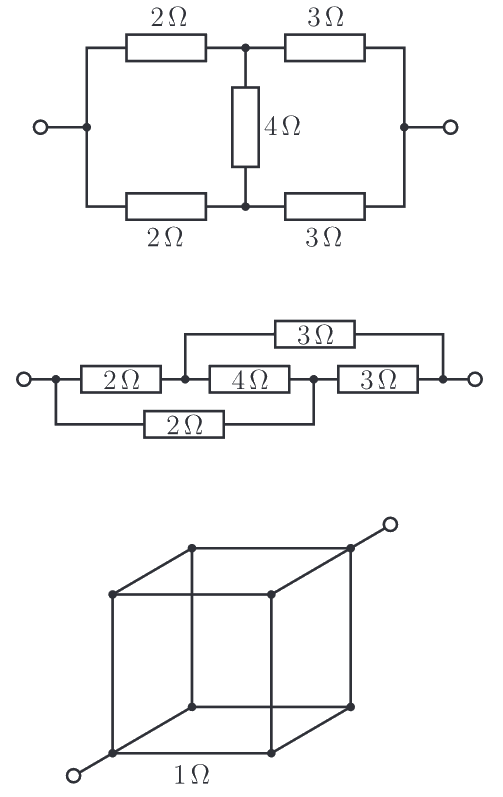
\includegraphics[width=0.6\textwidth]{S1 Figures/S1-23.png}
\end{center}
\end{solution}

\hypertarget{P24}{}
\begin{solution}{normal} % 24
Determine the resistance of the following circuit.
\begin{center}
    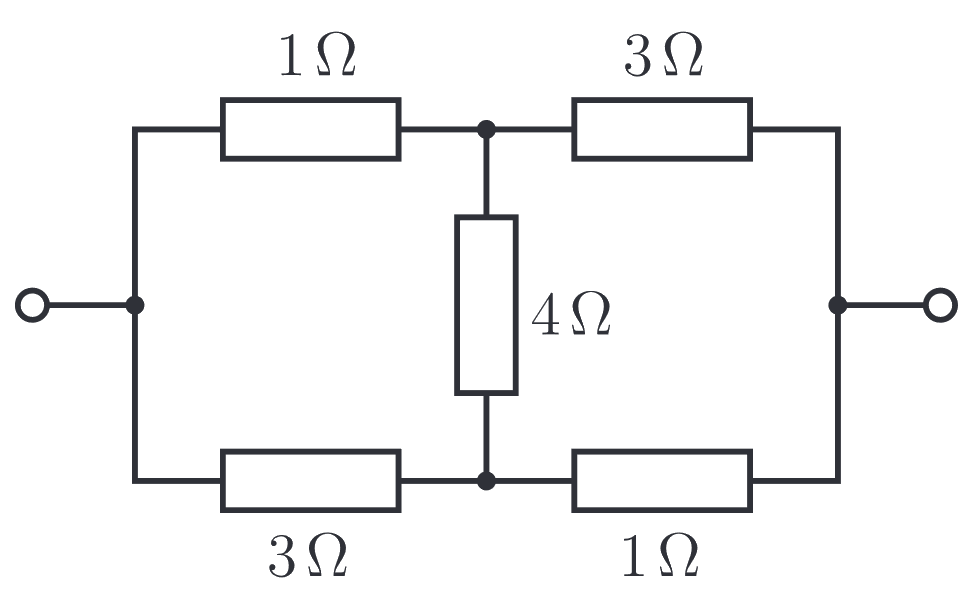
\includegraphics[width=0.55\textwidth]{S1 Figures/S1-24.png}
\end{center}
\end{solution}

\hypertarget{P25}{}
\begin{solution}{normal} % 25
Assuming ideal batteries, determine the currents through all resistors in the following circuit. (Similar to Kalda Circuits P12)
\begin{center}
    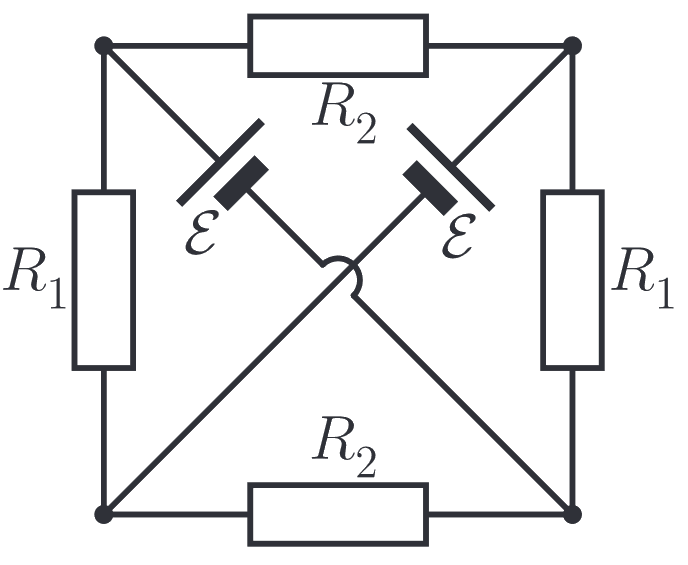
\includegraphics[width=0.4\textwidth]{S1 Figures/S1-25.png}
\end{center}
\end{solution}

\hypertarget{P26}{}
\begin{solution}{normal} % 26
Determine the resistance between any 2 terminals in the circuit shown below.
\begin{center}
    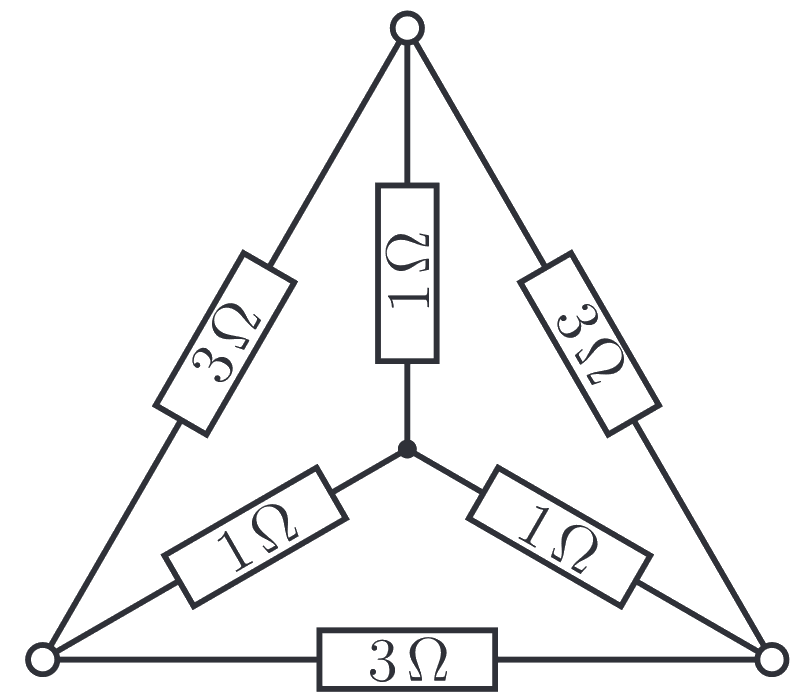
\includegraphics[width=0.45\textwidth]{S1 Figures/S1-26.png}
\end{center}
\end{solution}

\hypertarget{P27}{}
\begin{solution}{normal} % 27
Determine the reading of the ideal ammeter in the circuit below. (Kalda Circuits P36)
\begin{center}
    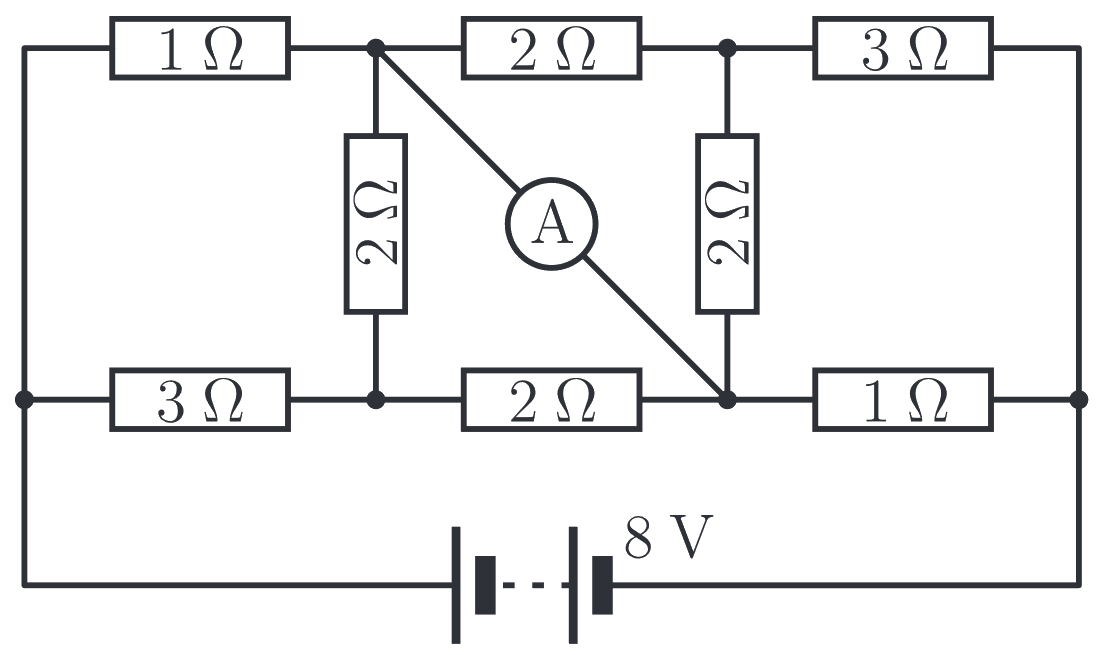
\includegraphics[width=0.6\textwidth]{S1 Figures/S1-27.png}
\end{center}
\end{solution}

\hypertarget{P28}{}
\begin{solution}{normal} % 28
Determine the readings on the ideal ammeter and ideal voltmeter in the following circuit.
\begin{center}
    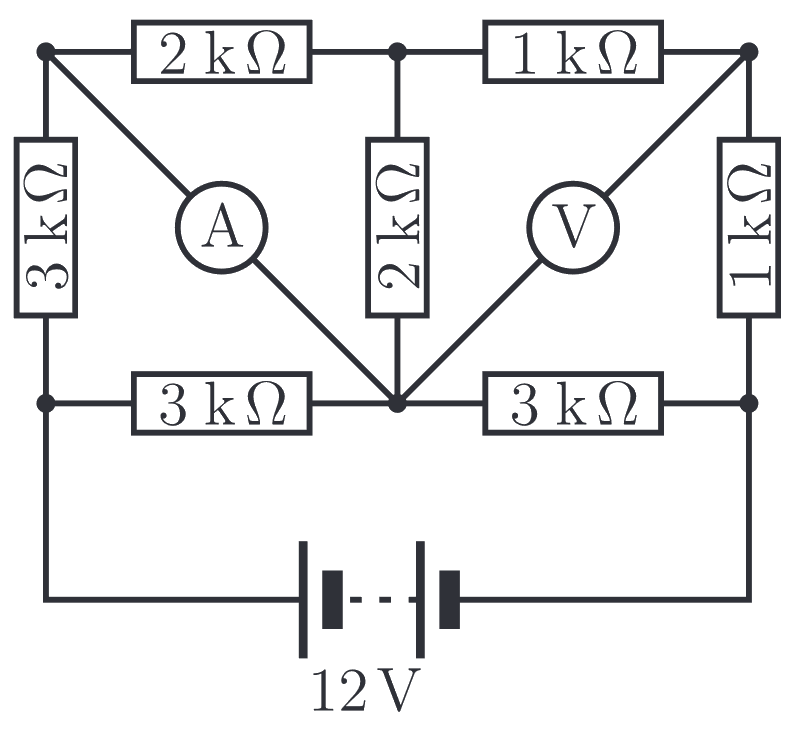
\includegraphics[width=0.45\textwidth]{S1 Figures/S1-28.png}
\end{center}
\end{solution}

\hypertarget{P29}{}
\begin{solution}{normal} % 29
Determine the resistance of the following infinite circuit. (Kalda Circuits P16)
\begin{center}
    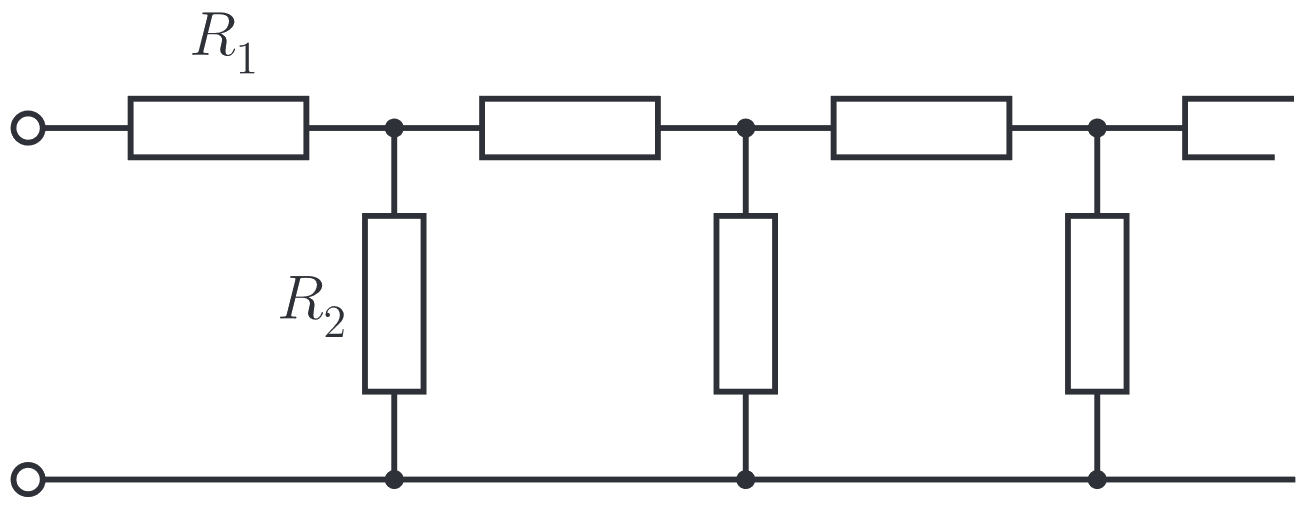
\includegraphics[width=0.7\textwidth]{S1 Figures/S1-29.png}
\end{center}
\end{solution}

\hypertarget{P30}{}
\begin{solution}{normal} % 30
Determine the electromotive force and internal resistance of the following system of batteries. (Kalda Circuits P17)
\begin{center}
    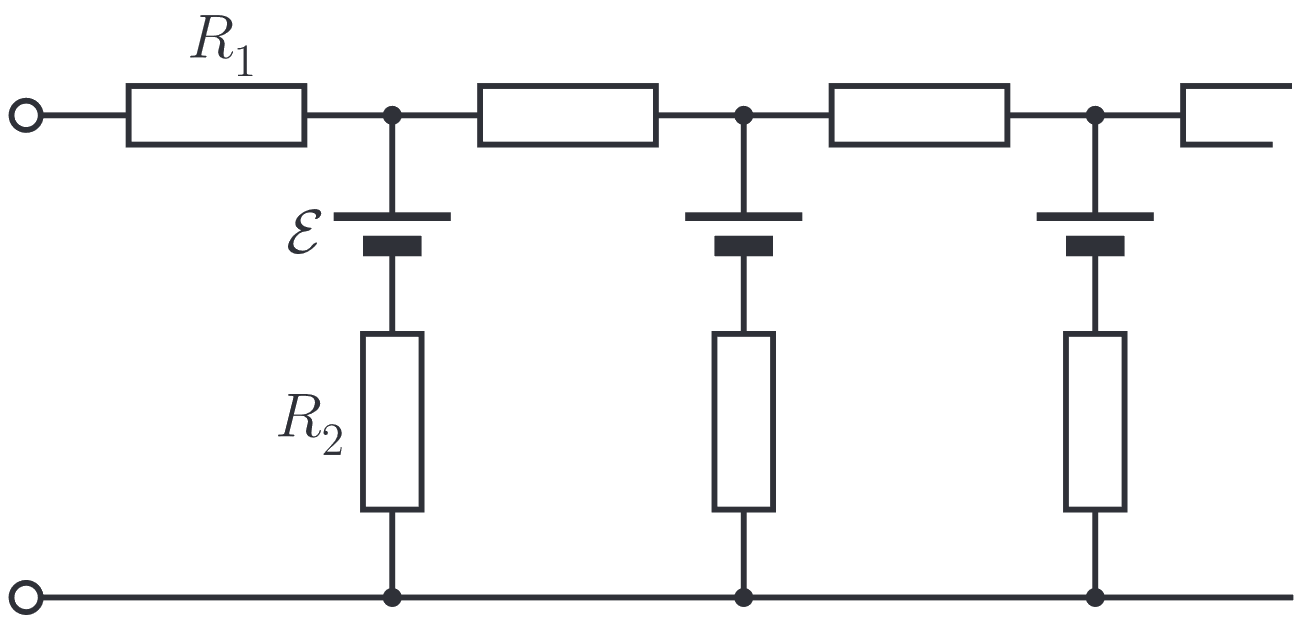
\includegraphics[width=0.7\textwidth]{S1 Figures/S1-30.png}
\end{center}
\end{solution}

\hypertarget{P31}{}
\begin{solution}{normal} % 31 ? Not really sure about the instructions part
Determine the resistance between two neigbouring nodes in an infinite triangular lattice, as shown in the figure below. The resistance of the wire connecting any two neighbouring nodes is $1\;\Omega$. \textit{Instructions:} Let $C$ be a node that is infinitely far from nodes $A$ and $B$. Now consider the currents flowing between these nodes.
\begin{center}
    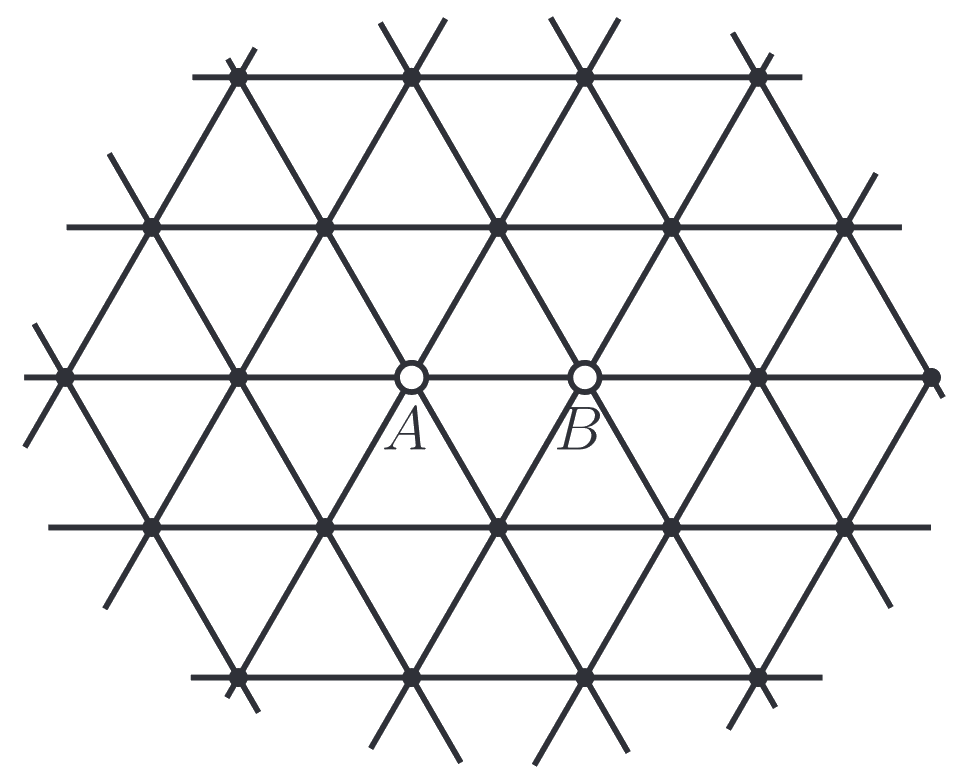
\includegraphics[width=0.5\textwidth]{S1 Figures/S1-31.png}
\end{center}
\end{solution}

\hypertarget{P32}{}
\begin{solution}{normal} % 32
Determine the resistance between two neighbouring nodes $A$ and $B$ of an infinite cubic lattice assuming that the edges of the lattice are made of wire, and the resistance of each edge is $1\;\Omega$. (Kalda Circuits P45)
\end{solution}

\hypertarget{P33}{}
\begin{solution}{normal} % 33
Solve Problem 31 if the wire connecting nodes A and B is cut (i.e. current cannot flow through that wire).
\end{solution}

\hypertarget{P34}{}
\begin{solution}{normal} % 34
How man times does the current through the battery change if the polarity of the polarity of the battery is reversed? All resistors are identical, diodes are ideal, and the internal resistance of the battery is negligible. (Kalda Circuits P44)
\begin{center}
    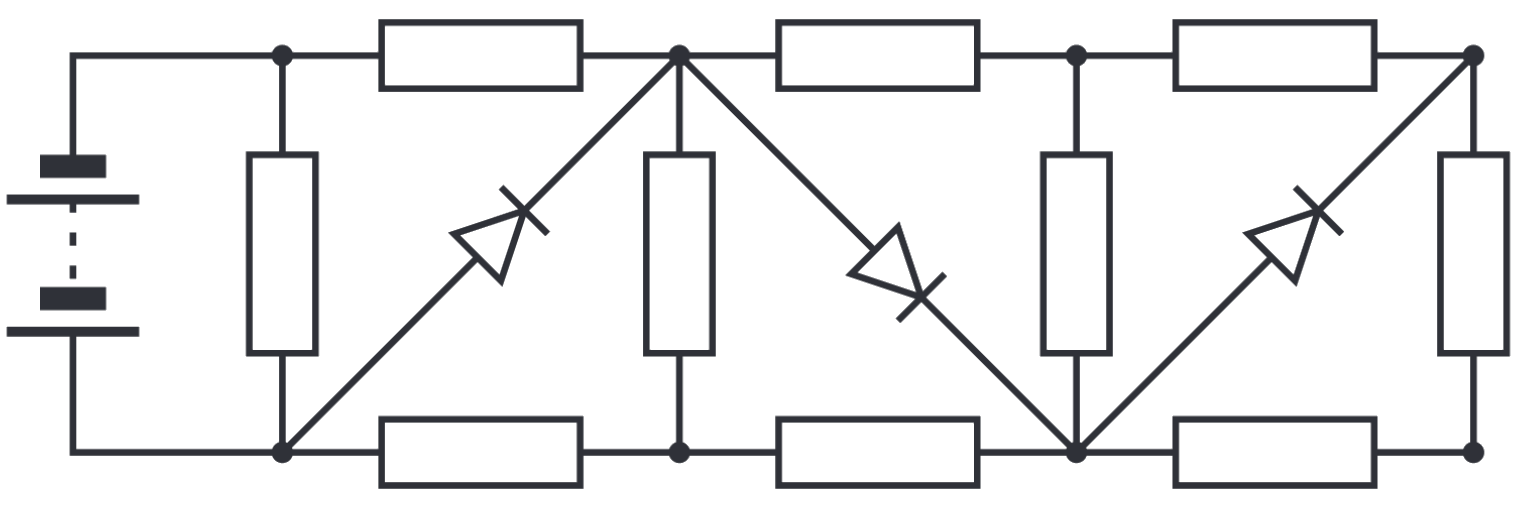
\includegraphics[width=0.8\textwidth]{S1 Figures/S1-34.png}
\end{center}
\end{solution}

\hypertarget{P35}{}
\begin{solution}{normal} % 35
Find the power dissipation on each of the diodes in the figure below. These diodes open at the forward voltage $V_0=1.0\;\text{V}$. It can be assumed that the diode voltage remains equal to $V_0$ for any forward current, and that for voltages less than $V_0$, there is no current through the diode, as shown in the figure below. The values of the resistances and of the electromotive force are given in the figure. (Kalda Circuits P29)
\begin{center}
    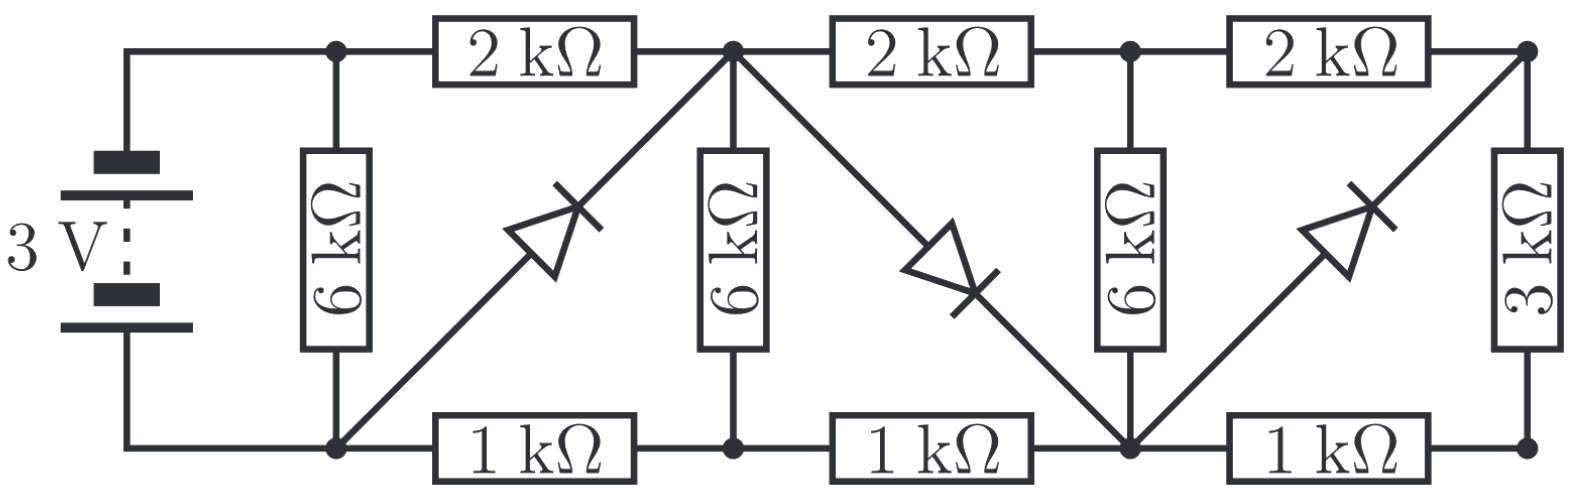
\includegraphics[width=0.8\textwidth]{S1 Figures/S1-35-1.png}
\end{center}
\begin{center}
    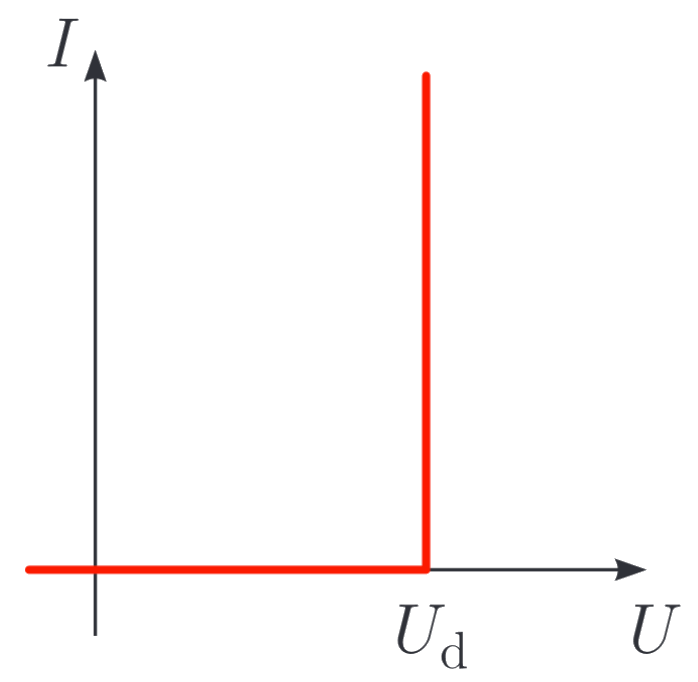
\includegraphics[width=0.4\textwidth]{S1 Figures/S1-35-2.png}
\end{center}
\end{solution}

\hypertarget{P36}{}
\begin{solution}{normal} % 36
Find the current in the circuit given below; the $I(V)$ dependence of the diode is shown in graph. (Kalda Circuits P24)
\begin{center}
    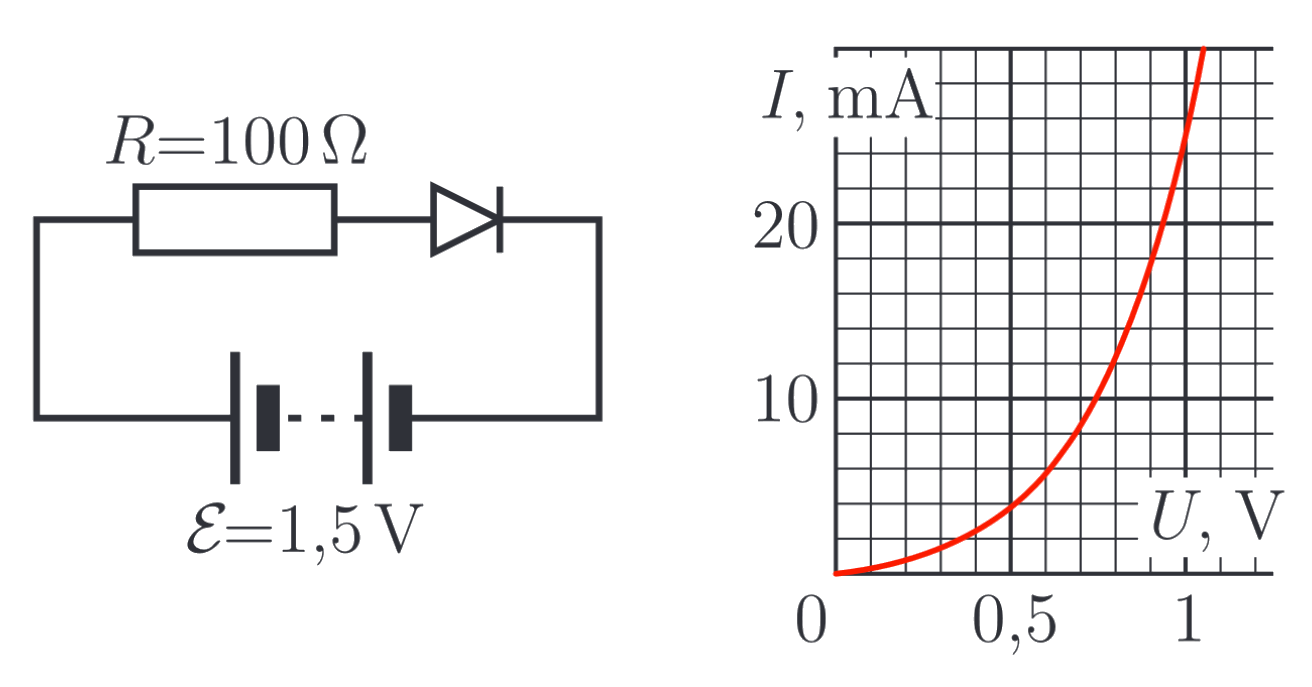
\includegraphics[width=0.75\textwidth]{S1 Figures/S1-36.png}
\end{center}
\end{solution}

\hypertarget{P37}{}
\begin{solution}{normal} % 37
Determine the current flowing through diode $D_2$ in the circuit below. The diodes are identical and have $I(V)$ dependence identical to the diode in Problem 36.
\begin{center}
    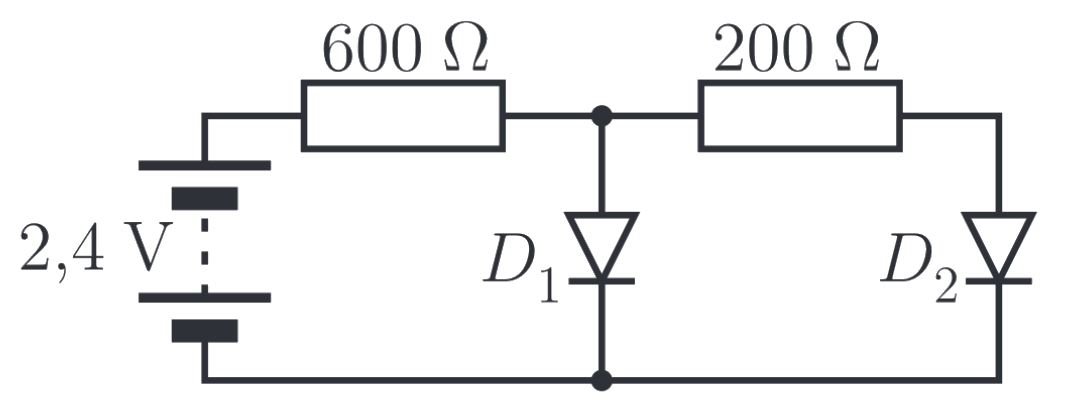
\includegraphics[width=0.6\textwidth]{S1 Figures/S1-37.png}
\end{center}
\end{solution}

\hypertarget{P38}{}
\begin{solution}{normal} % 38
The figure below shows the $I(V)$ dependence of the lamp, which is connected to the circuit as shown in the diagram below. How much power is dissipated by the lamp?
\begin{center}
    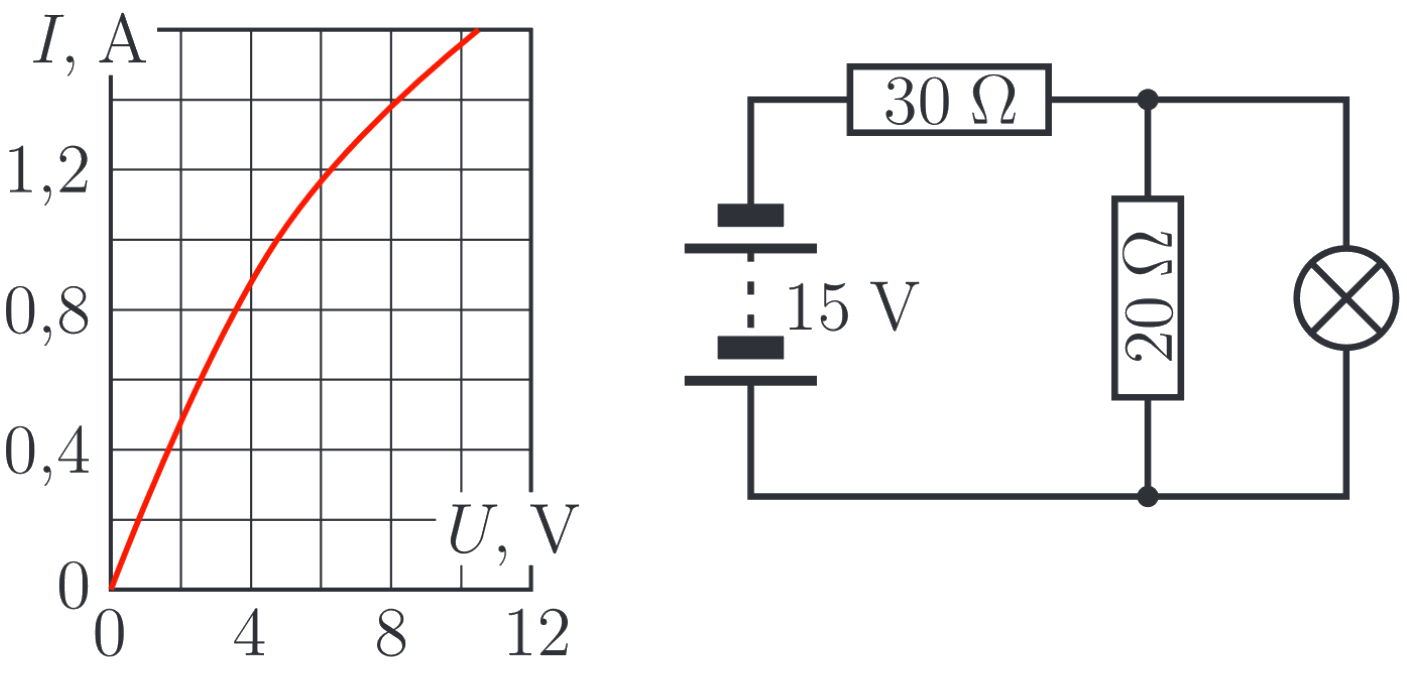
\includegraphics[width=0.75\textwidth]{S1 Figures/S1-38.png}
\end{center}
\end{solution}

\hypertarget{P39}{}
\begin{solution}{normal} % 39 ? unsure about translation
The $I-V$ curve of a thyristor is shown in the graph below. The thyristor is connected in series with a resistor of resistance $R$. What minimum voltage $U_0$ must be applied to the circuit for the thyristor to open (i.e. the current in the circuit increases exponentially)? Sketch the change in current in the circuit as the voltage applied increases linearly from $0$ to $U_0$ and back to $0$.
\begin{center}
    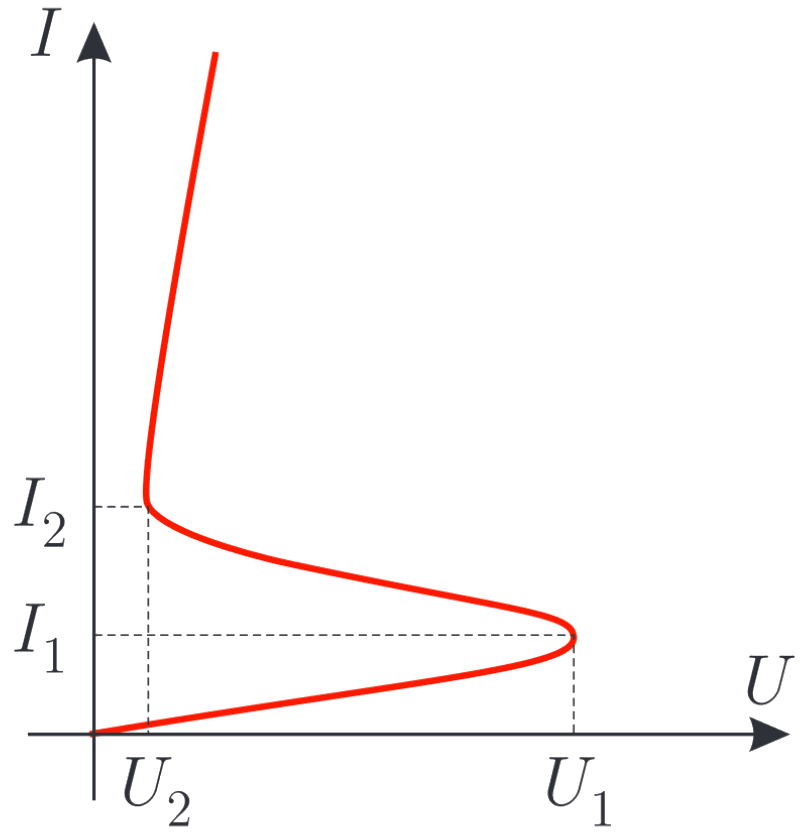
\includegraphics[width=0.4\textwidth]{S1 Figures/S1-39.png}
\end{center}
\end{solution}

\hypertarget{P40}{}
\begin{solution}{normal} % 40
In the figure below, the circuit of a simple tunnel-diode-based amplifier is given. Find the amplification factor for small-amplitude input signals using the following values. (Similar to Kalda Circuits P25)
\begin{center}
    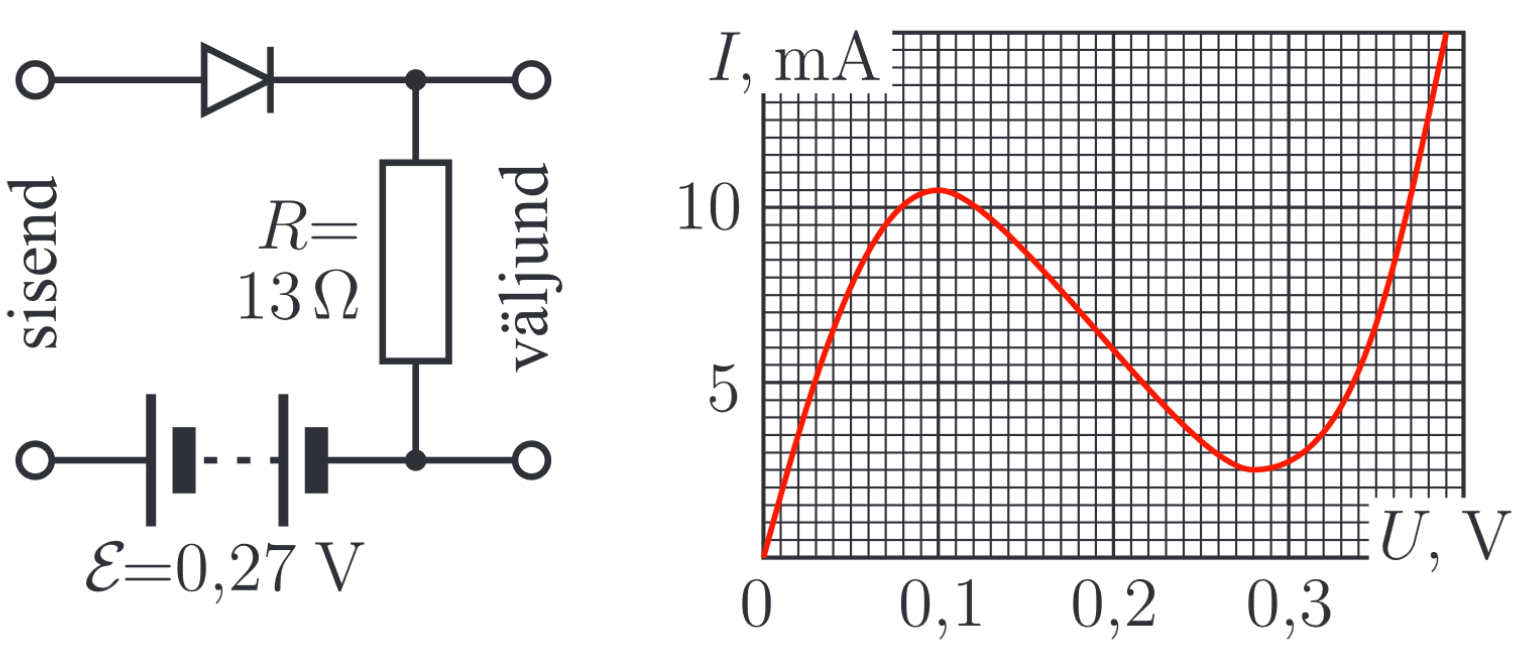
\includegraphics[width=0.7\textwidth]{S1 Figures/S1-40.png}
\end{center}
\end{solution}

\hypertarget{P41}{}
\begin{solution}{normal} % 41
To determine the current in a circuit, two ammeters with different measuring ranges are connected, one at a time. The ammeter with a measuring range of $10\;\text{mA}$ has a current reading of $2.95\;\text{mA}$ and the ammeter with a measuring range of $3\;\text{mA}$ has a current reading of $2.90\;\text{mA}$. What is the current in the circuit without an ammeter present? Assume that we are using a magnetoelectric ammeter with internal resistance inversely proportional to the measuring range. \textit{Note:} As the difference between the ammeter readings is relatively small, a linear approximation may be used and the change in current due to the additional resistance in the circuit (not due to the ammeter) can be considered to be proportional to the magnitude of the resistance.
\end{solution}

\hypertarget{P42}{}
\begin{solution}{normal} % 42
Show that if the resistance of an incandescent lamp is proportional to its (absolute) temperature, the current-voltage characteristic of the lamp is $I\propto U^{3/5}$.
\end{solution}

\hypertarget{P43}{}
\begin{solution}{normal} % 43
The label on a filament lamp  reads: $26\;\text{V},\;0.12\;\text{A}$. At room temperature, the resistance of the filament was measured to be $R_0=24\;\Omega$. Determine the length, diameter, and operating temperature of the filament. The filament is made of tungsten and has resistivity $\rho_0=5.3\times10^{-8}\;\Omega\;\text{m}$.
\end{solution}

\hypertarget{P44}{}
\begin{solution}{normal} % 44
The filament in a halogen light bulb is $5\;\text{cm}$ long. The filament is made of tungsten wire with density $19300\;\text{kg}/\text{m}^3$ and specific heat capacity $134\;\text{J}/(\text{kg}\cdot\text{K})$, which can be considered to be constant over the given temperature range. The resistivity of tungsten as a function of temperature is shown in the graph below. An excessive DC voltage of $120\;\text{V}$ is applied to the bulb. How long does it take to reach its melting point of $3410\degree\text{C}$?
\begin{center}
    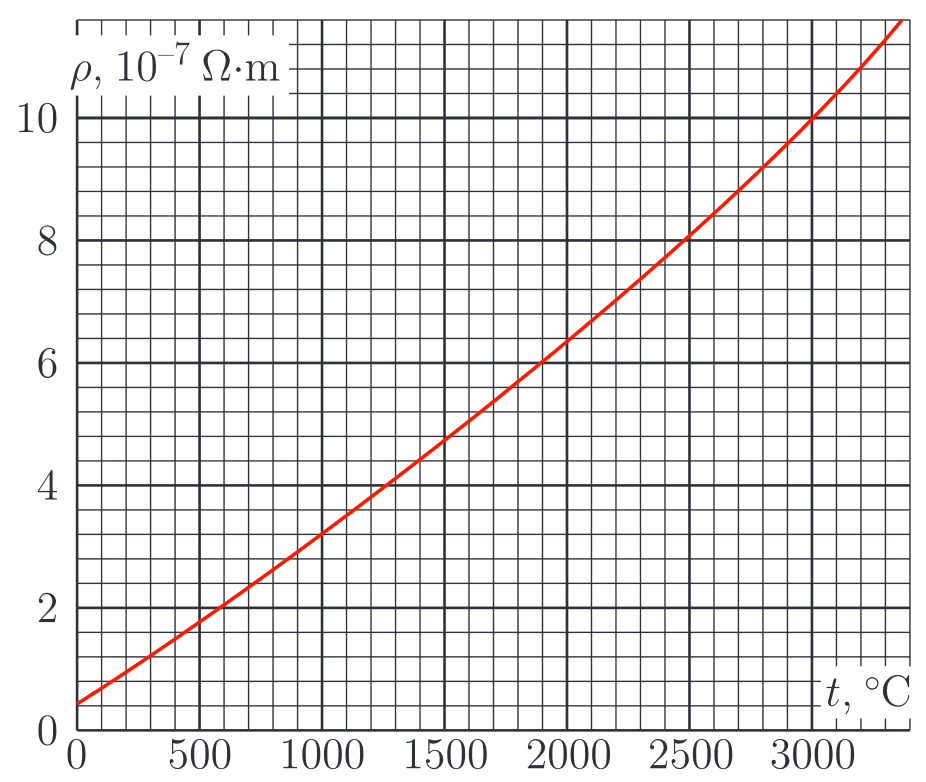
\includegraphics[width=0.7\textwidth]{S1 Figures/S1-44.png}
\end{center}
\end{solution}

\newpage
\section{DC Circuits With Capacitors}
\hypertarget{P45}{}
\begin{solution}{normal} % 45
In the circuit shown below, all capacitors are initially uncharged. a) Find the current through the battery immediately after closing switch $K$. b) What will be the charges on each of the capacitors after a steady state has been reached?
\begin{center}
    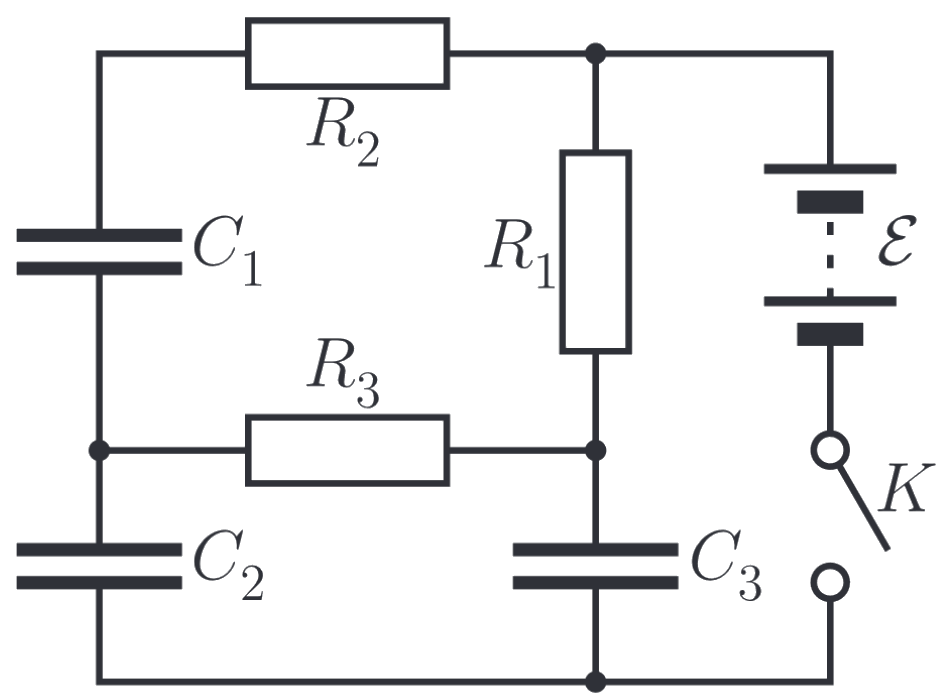
\includegraphics[width=0.43\textwidth]{S2 Figures/S2-45.png}
\end{center}
\end{solution}

\hypertarget{P46}{}
\begin{solution}{normal} % 46
A resistor $R$ and a capacitor $C$ are connected in series with a DC voltage source with emf $\mathcal{E}$. The capacitor was initially uncharged. Find the power dissipated by the resistor. (Kalda Circuits P57)
\end{solution}

\hypertarget{P47}{}
\begin{solution}{normal} % 47
A capacitor with capacitance $C=10\;\mu\text{F}$ is charged to a potential difference of $U_0=6\;\text{V}$. Then, a switch completes a circuit containting only the capacitor and a diode with current-voltage characteristic (let $U_d=1\;\text{V}$) shown in the graph below. How much energy is released at the switch in the form of a flash (i.e. arcing), if we neglect heat dissipation in the wires?
\begin{center}
    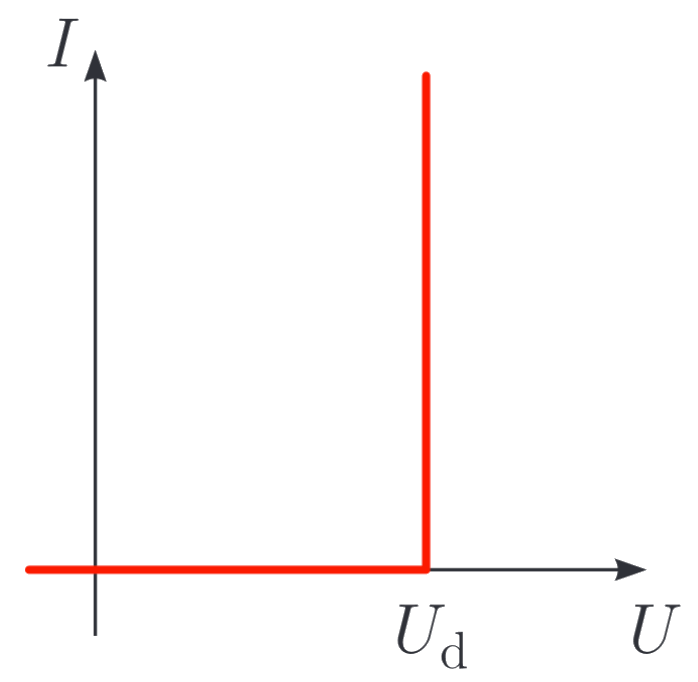
\includegraphics[width=0.32\textwidth]{S1 Figures/S1-35-2.png}
\end{center}
\end{solution}

\hypertarget{P48}{}
\begin{solution}{normal} % 48
Prove that the formula for the total capacitance of capacitors in series is given by
$$C=\left(\dfrac{1}{C_1}+\dfrac{1}{C_2}+\cdots\right)^{-1}$$
(Kalda Circuits P60)
\end{solution}

\hypertarget{P49}{}
\begin{solution}{normal} % 49
Three identical uncharged capacitors of capacitance $C$ are connected in series. A battery of emf $\mathcal{E}$ is connected to the circuit as shown. When the capacitors are fully charged, they are disconnected from the voltage source and connected to two identical resistors of resistance $R$ as shown in the circuit below. Determine the power dissipated by each resistor. (Kalda Circuits P61)
\begin{center}
    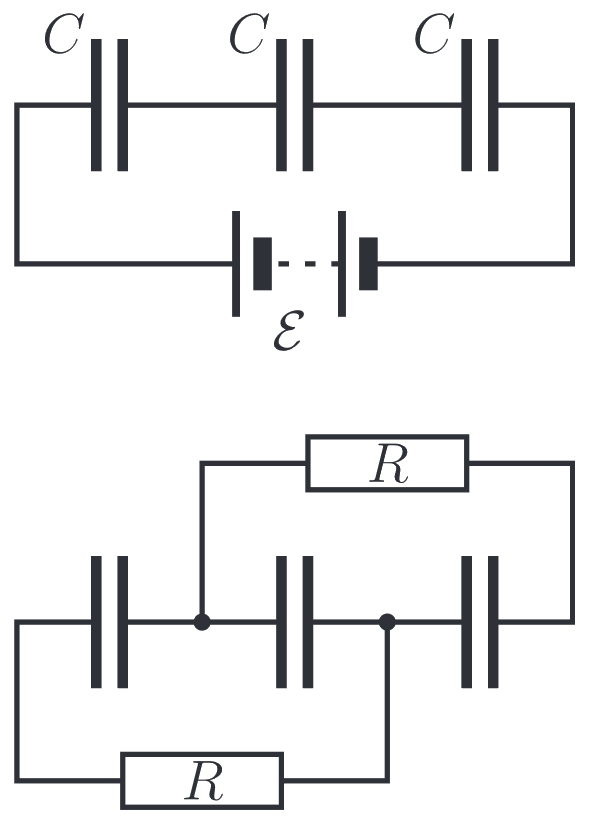
\includegraphics[width=0.33\textwidth]{S2 Figures/S2-49.png}
\end{center}
\end{solution}

\hypertarget{P50}{}
\begin{solution}{normal} % 50
In the circuit below, switch $K$ has been open for a long time. How much heat is dissipated at $R_1$ after closing the switch?
\begin{center}
    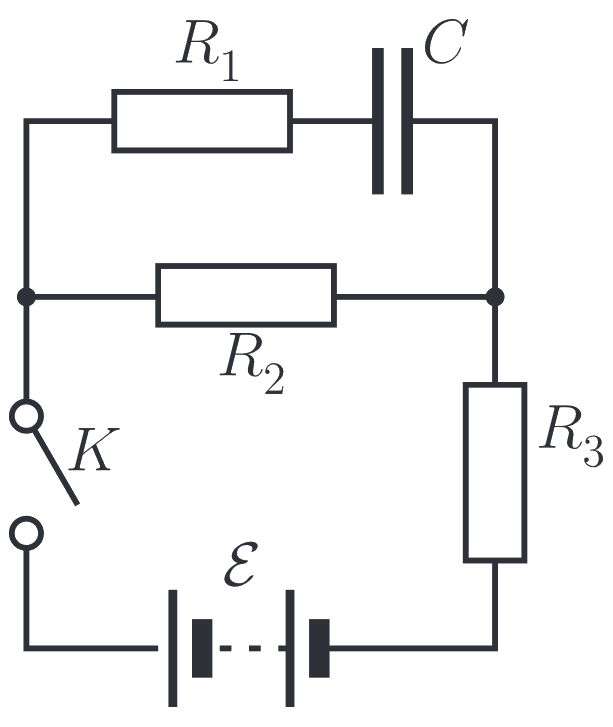
\includegraphics[width=0.33\textwidth]{S2 Figures/S2-50.png}
\end{center}
\end{solution}

\hypertarget{P51}{}
\begin{solution}{normal} % 51
Two parallel metal plates of area $100\;\text{cm}^2$ are spaced $1\;\text{mm}$. The plates are connected to a voltage source of emf $12\;\text{V}$. How much force is required to hold the plates in place? \textit{Note:} Use two different methods to solve the problem: in one case the voltage source is permanently connected; in the other case, once the capacitor is fully charged, the source is disconnected after the capacitor is fully charged. In either case, the answer should be the same. 
\end{solution}

\hypertarget{P52}{}
\begin{solution}{normal} % 52
A capacitor consists of two semicircular parallel plates that can rotate frictionlessly around a common axis (see the figure below). The distance between the plates is $d$ and each plate has radius $R$ ($d\ll R$). Determine the torque applied by the lower plate on the upper plate when the angle of overlap of the two plates is $\alpha$ ($\alpha\gg d/R$) and a voltage $U$ is applied to the plates.
\begin{center}
    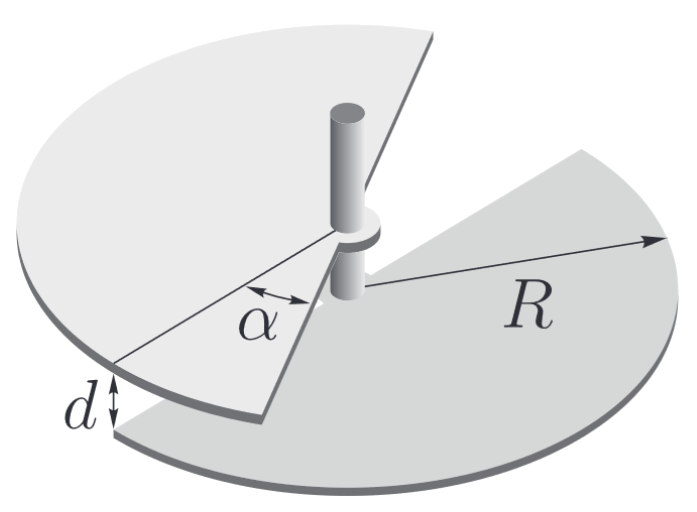
\includegraphics[width=0.32\textwidth]{S2 Figures/S2-52.png}
\end{center}
\end{solution}

\hypertarget{P53}{}
\begin{solution}{normal} % 53 ? unsure about translation
Find the minimum force necessary to remove a dielectric completely filling the space between two plates of a capacitor if the width of the plate is $a$, the distance between the plates is $d$, the dielectric constant is $\kappa$, and a voltage $U$ is applied to the capacitor.
\end{solution}

\hypertarget{P54}{}
\begin{solution}{normal} % 54
A parallel plate capacitor has plates spaced a distance $d$ apart. A voltage $U$ is applied across the capacitor. The capacitor is placed, along its lower edge, in a liquid with dielectric constant $\kappa$ and density $\rho$. How high does the liquid rise between the plates of the capacitor? Do not consider surface tension.
\end{solution}

\hypertarget{P55}{}
\begin{solution}{normal} % 55
The space between the plates of a capacitor is filled with an insulator with dielectric constant $5$ and resistivity $10^{12}\;\Omega\;\text{m}$. Find the time constant of the capacitor.
\end{solution}

\hypertarget{P56}{}
\begin{solution}{normal} % 56
The figure below shows the schematic for a simple timer. Assume that the inputs of the comparator consume practically no current. The capacitor is initially uncharged. How long does it take for the alarm to go off after closing the switch? \textit{Note:} The triangular circuit element is a comparator - a device that emits a signal (which in turn triggers an alarm) as soon as the potential difference between its inputs becomes positive. Dashed lines indicate connections between the comparator and alarm, but this is not required to solve the problem.
\begin{center}
    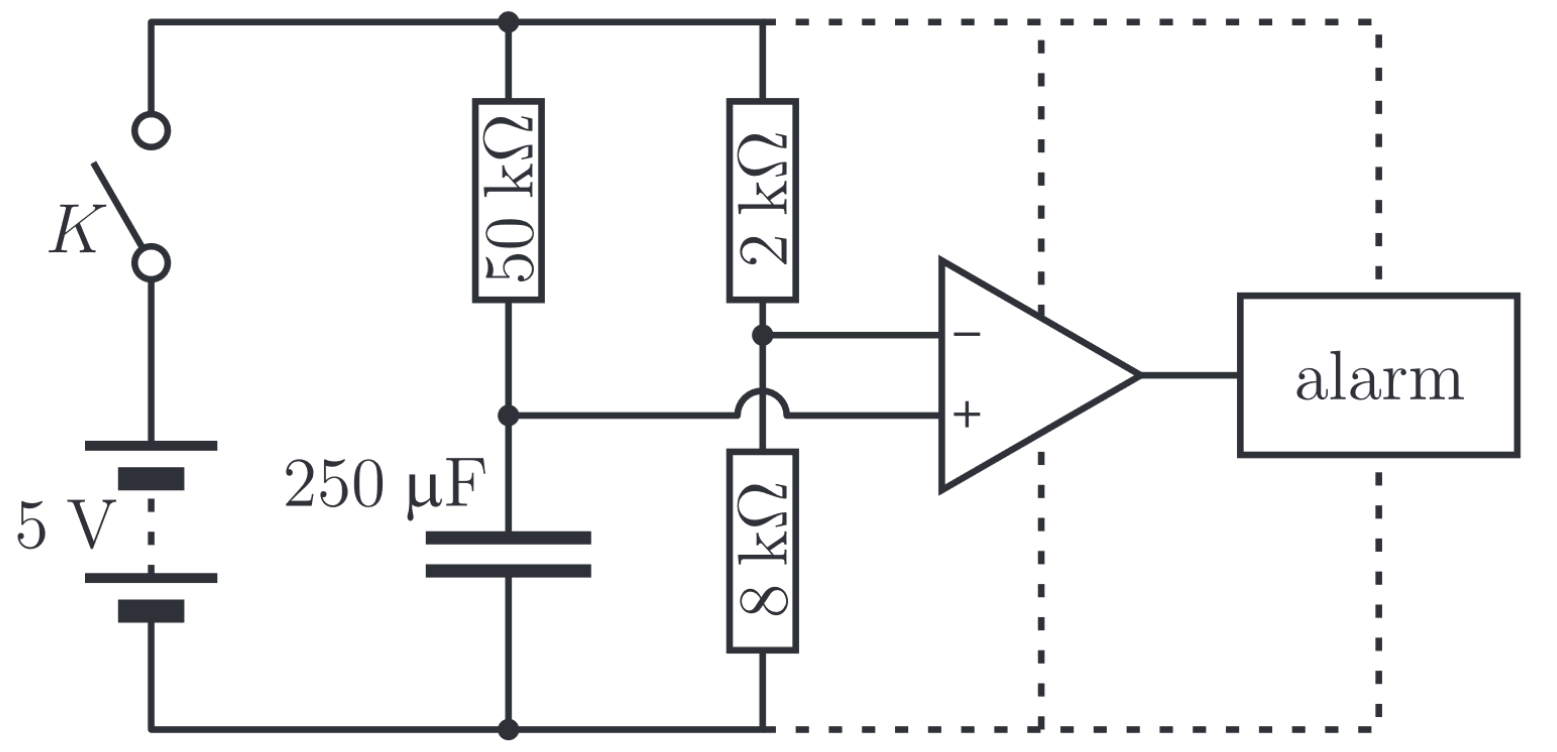
\includegraphics[width=0.53\textwidth]{S2 Figures/S2-56.png}
\end{center}
\end{solution}

\hypertarget{P57}{}
\begin{solution}{normal} % 57
Find the time constant of the capacitor in the diagram below after closing switch $K$.
\begin{center}
    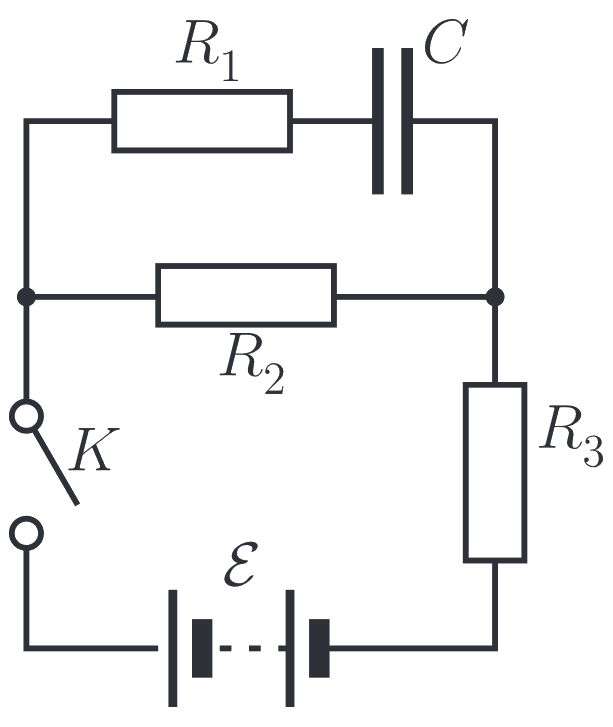
\includegraphics[width=0.33\textwidth]{S2 Figures/S2-50.png}
\end{center}
\end{solution}

\hypertarget{P58}{}
\begin{solution}{normal} % 58
An AC voltage as shown below is applied to a circuit consisting of a resistor and a capacitor connected in series. Determine the power dissipated by the resistor in the following cases: a) $T\ll RC$; b) $T\gg RC$.
\begin{center}
    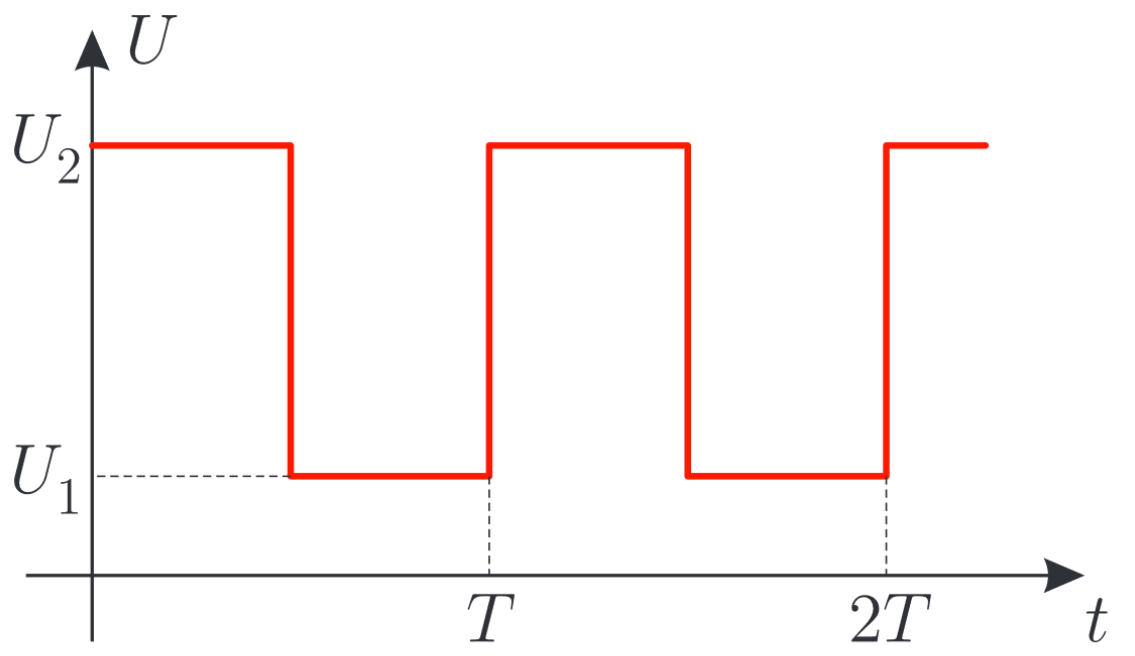
\includegraphics[width=0.5\textwidth]{S2 Figures/S2-58.png}
\end{center}
\end{solution}

\hypertarget{P59}{}
\begin{solution}{normal} % 59
A time-dependent current flows through a circuit consisting of a resistor and a capacitor connected in series. Determine the amplitude of voltage fluctuations in the capacitor in the following cases: a) $T\ll RC$; b) $T\gg RC$.
\begin{center}
    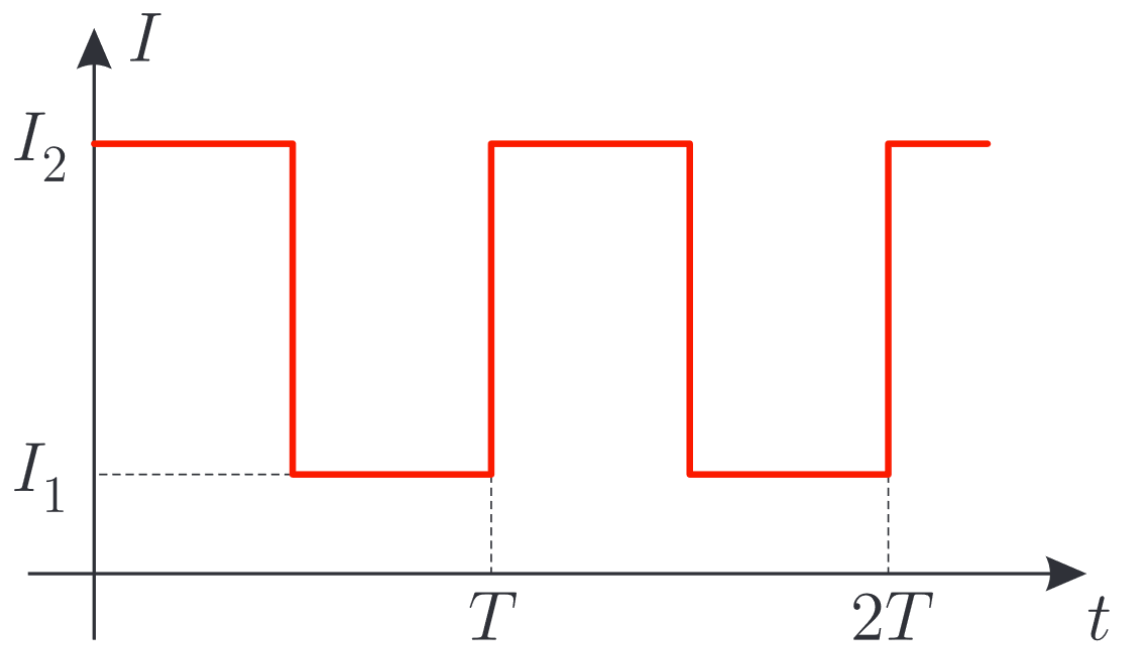
\includegraphics[width=0.5\textwidth]{S2 Figures/S2-59.png}
\end{center}
\end{solution}

\hypertarget{P60}{}
\begin{solution}{normal} % 60
A boy wants to build decorative lights using 50 LEDs, to be fed by AC voltage $V=V_0\cos(2\pi\nu t)$, with $V_0= 220\;\text{V}$ and $\nu= 50\;\text{Hz}$.  The circuit he plans to use is given below. The voltage of his LEDs can be taken to be equal to $3\;\text{V}$ (it remains constant for a wide range of forward currents); the nominal current is $20\;\text{mA}$. Find a) the optimal value of the resistor $R$ (ensuring a nominal operation of the diodes) and the power it dissipates, and b) the minimal value of the capacitance $C$, if the current fluctuations need to be less than 5\%. The rectifying diode $D$ can be considered to be ideal. (Kalda Circuits P75)
\begin{center}
    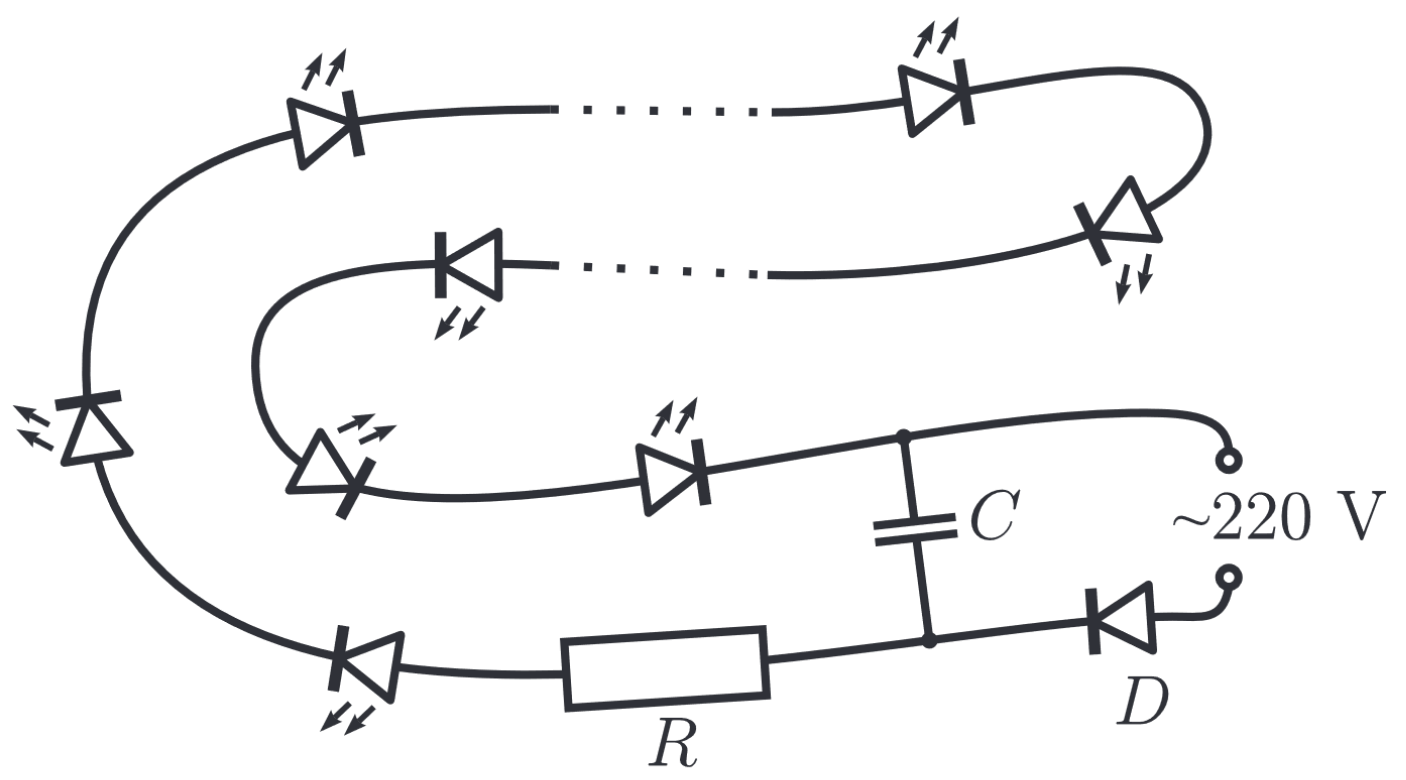
\includegraphics[width=0.7\textwidth]{S2 Figures/S2-60.png}
\end{center}
\end{solution}

\newpage
\section{Electrostatics}
\hypertarget{P61}{}
\begin{solution}{normal} % 61
Four identical point charges of charge $q$ lie on the vertices of a square with side length $L$. Determine the magnitude of the force acting on the charges.
\end{solution}

\hypertarget{P62}{}
\begin{solution}{normal} % 62
There are fixed point charges of $q,2q,3q,\dots,12q\;(q>0)$ on a clock face, with each of the charges on their respective hour. What time (hours and minutes) does the electric field vector at the center of the clock point towards? \textit{Tip:} Use symmetry and the fact that the sum of the vectors does not depend on the order of the additions.
\end{solution}

\hypertarget{P63}{}
\begin{solution}{normal} % 63
Two point charges $q_1$ and $q_2$ are located a distance $L$ from each other. Where should a third charge be placed and what should its magnitude be in order to balance the first two charges? \textit{Tip:} In order to write a general answer for this problem, you should define a coordinate axes to determine the locations of the charges and carefully consider the signs of the charges.
\end{solution}

\hypertarget{P64}{}
\begin{solution}{normal} % 64 ? unsure about translation
A third point charge is placed in between two identical fixed point charges. Does that charge remain in stable equilibrium if its charge has opposite sign to the two extreme charges? \textit{Note:} Equilibrium stability means that a small deviation from the equilibrium position results in a force that directs the body back toward the equilibrium position.
\end{solution}

\hypertarget{P65}{}
\begin{solution}{normal} % 65
Two identical point charges of charge $q$ are located a distance $2d$ from each other. Find the maximum magnitude of the electric field on the perpendicular bisector of the line connecting these charges. \textit{Note:} If we plot the dependence $y=f(x)$, then the point of the graph where $f(x)$ acquires its maximum value is where the tangent to the graph is momentarily horizontal (i.e. its slope is zero or $f'(x)=0$).
\end{solution}

\hypertarget{P66}{}
\begin{solution}{normal} % 66
Prove that it is not possible to generate an electrostatic field in which the point charge remains in stable equilibrium. \textit{Note:} This is known as Earnshaw's theorem.
\end{solution}

\hypertarget{P67}{}
\begin{solution}{normal} % 67
Find the electric field of a uniformly charged infinite plane having surface charge density $\sigma$.
\end{solution}

\hypertarget{P68}{}
\begin{solution}{normal} % 68
Find the field created by a parallel plate capacitor with surface charge densities $\pm \sigma$. Also find the force per unit area acting between the plates, or namely, the electrostatic pressure between the plates. \textit{Note:} From here on, unless otherwise indicated, assume that the dimensions of the capacitor plates are much larger than their separation distance.
\end{solution}

\hypertarget{P69}{}
\begin{solution}{normal} % 69 ? unsure about translation
In nice weather, an electric field of magnitude $150\;\text{V}/\text{m}$ is directed downwards near the Earth's surface. The field strength decreases with height and is $100\;\text{V}/\text{m}$ at a height of $100\;\text{m}$. Determine the average charge density in the atmosphere.
\end{solution}

\hypertarget{P70}{}
\begin{solution}{normal} % 70
Find the strength of the electric field generated by a thin, straight infinitely long wire at a distance $r$ from it, if the linear charge density along the wire is $\lambda$.
\end{solution}

\hypertarget{P71}{}
\begin{solution}{normal} % 71
Prove that the electric field inside a uniformly charged non-conducting hollow shell is zero.
\end{solution}

\hypertarget{P72}{}
\begin{solution}{normal} % 72
Find the electric field due to a uniformly charged non-conducting solid sphere of radius $R$ having volumetric charge density $\rho$.
\end{solution}

\hypertarget{P73}{}
\begin{solution}{normal} % 73
Find the strength of the electric field due to a non-conducting infinitely long charged cylinder at a distance r from the axis of the cylinder. The volumetric charge density of the cylinder is $\rho$ and the radius of the cylinder is $R$.
\end{solution}

\hypertarget{P74}{}
\begin{solution}{normal} % 74
A thin planar electrode has a small circular opening of radius $a$. There is a uniform electric field $\textbf{\textit{E}}_1$ one one side of the electrode and a uniform electric field $\textbf{\textit{E}}_2$ on the other side (see the figure below). A beam of electrons is passed through the circular opening at a distance $z_1$ from the electrode and refocuses on the other side at a distance $z_2$ from the electrode. Assume that particle energy $eU_0\gg eE_1z_1,eE_2z_2$ and $a\ll z_1,z_2$. Show that under these conditions the "lens formula" $1/z_1+1/z_2=(E_1-E_2)/(4U_0)$ holds. \textit{Note:} in the immediate vicinity of the opening the field is non-uniform. To estimate the radial component of the electric field in this region, apply Gauss' Law to a short coaxial cylinder passing through the hole.
\begin{center}
    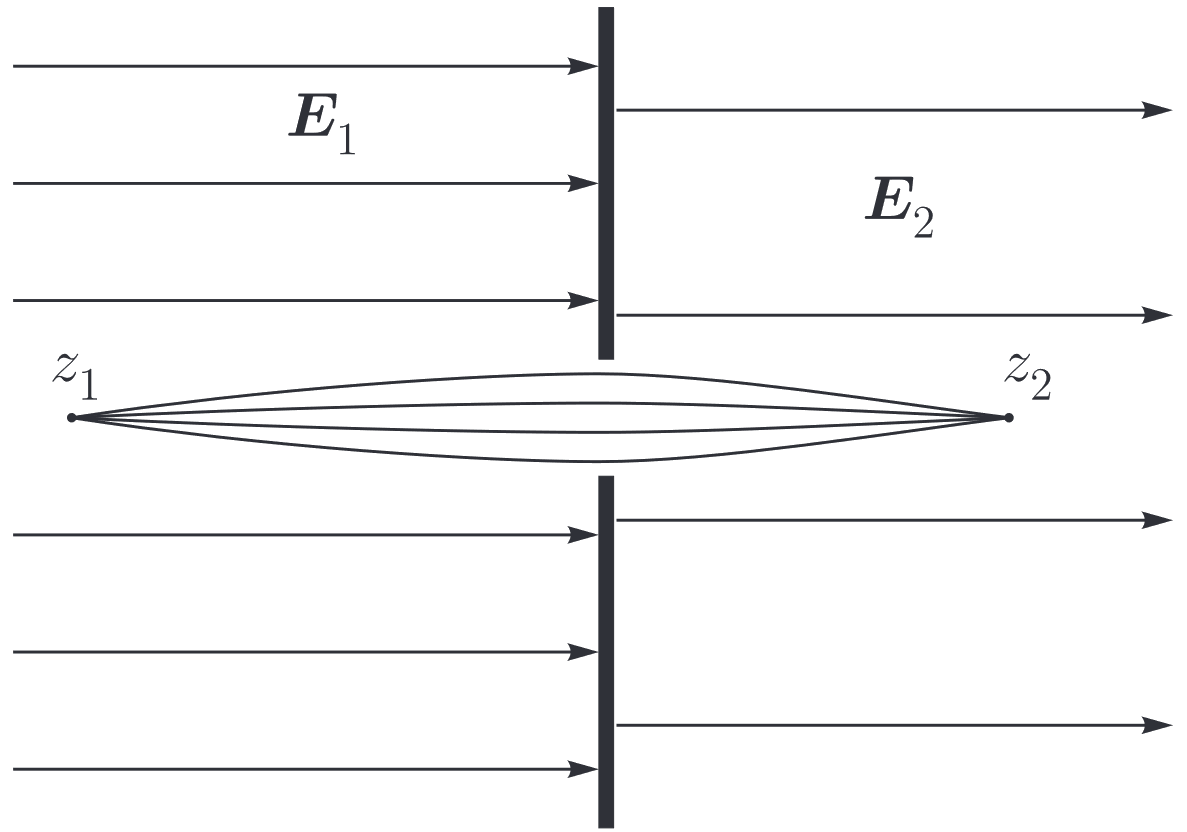
\includegraphics[width=0.5\textwidth]{S3 Figures/S3-74.png}
\end{center}
\end{solution}

\hypertarget{P75}{}
\begin{solution}{normal} % 75
a) Determine the electric field due to two non-conducting charged spheres of radius $R$ in their region of overlap. The volumetric charge densities of the spheres is $\pm \rho$ and the distance between the centres of the spheres is $d$.  b) Solve part a) if the two spheres are replaced by infinitely long parallel cylinders.
\begin{center}
    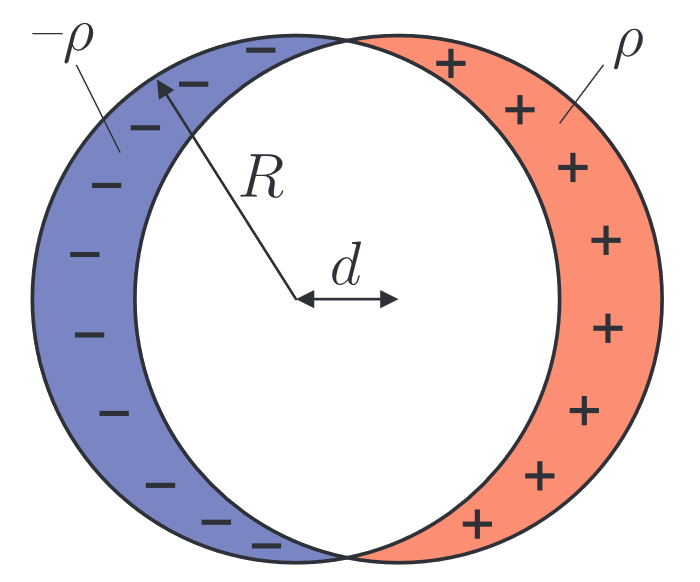
\includegraphics[width=0.4\textwidth]{S3 Figures/S3-75.png}
\end{center}
\end{solution}

\hypertarget{P76}{}
\begin{solution}{normal} % 76
Consider a uniformly charged sphere of charge density $\rho$. Inside this sphere is a spherical cavity located at a position $\textbf{\textit{r}}_0$ relative to the center of the sphere. Determine the electric field in the cavity.
\end{solution}

\hypertarget{P77}{}
\begin{solution}{normal} % 77
Show that the force acting between two spheres with uniform charge distribution is the same as the force between two point charges (i.e. $Q_1Q_2/(4\pi\varepsilon_0r^2)$), where $Q_1$ and $Q_2$ are the total charges on the spheres and $r$ is the distance between their centers.
\end{solution}

\hypertarget{P78}{}
\begin{solution}{normal} % 78
Determine the force between a uniformly charged infinitely long cylinder and a uniformly charged sphere. The linear charge density of the cylinder is $\lambda$, the total charge found on the sphere is $Q$ and $r$ is the distance from the centre of the sphere to the axis of the cylinder.
\end{solution}

\hypertarget{P79}{}
\begin{solution}{normal} % 79
Find the electrostatic pressure acting on the surface of a uniformly charged sphere if the surface charge density of the sphere is $\sigma$.
\end{solution}

\hypertarget{P80}{}
\begin{solution}{normal} % 80
Find the force exerted by one hemisphere of a non-conducting uniformly charged sphere having charge $Q$ and radius $R$ on the other hemisphere. \textit{Note:} This problem is also in Griffiths.
\end{solution}

\hypertarget{P81}{}
\begin{solution}{normal} % 81
Determine the electric field at a distance $r$ along the central axis of a dipole.
\end{solution}

\hypertarget{P82}{}
\begin{solution}{normal} % 82
Prove expression 4 for an electric dipole. \textit{Note:} Use the results of the previous problem to treat an arbitrarily oriented dipole as a superposition of two perpendicular dipoles. Essentially, this means adding additional fictitious charges $\pm q$ to a suitable points in space.
\begin{center}
    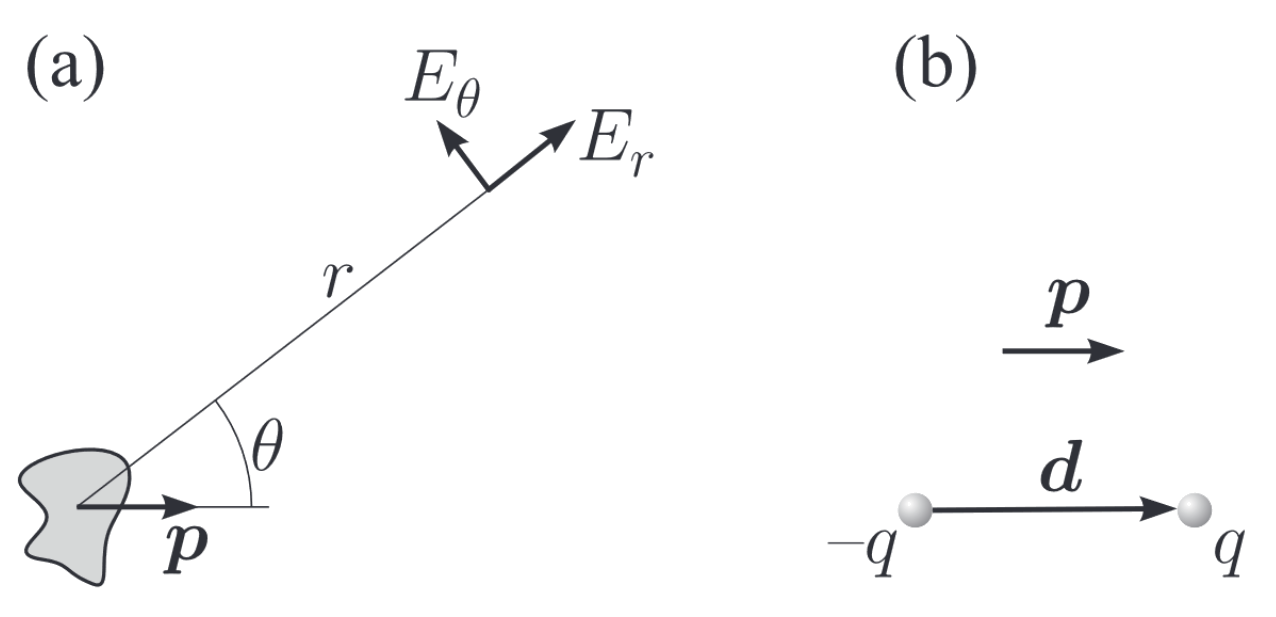
\includegraphics[width=0.5\textwidth]{S3 Figures/S3-82.png}
\end{center}
\blfootnote{Expression 4 (also see the figure above) gives $$E_r=\dfrac{2p\cos\theta}{4\pi\varepsilon_0r^3},\;\;\;E_\theta=\dfrac{p\sin\theta}{4\pi\varepsilon_0r^3}$$ where the quantity $\textbf{\textit{p}}=\sum q_i\textbf{\textit{r}}_i$ is known as the dipole moment of a system of charges}
\end{solution}

\hypertarget{P83}{}
\begin{solution}{normal} % 83
A parallel plate capacitor located in a vacuum is formed with two metal plates of area $S$. The capacitor is then charged to a voltage $U$. Determine the strength of the electric field in the plane of the plates at a distance $r$ from the plates, where $r$ is much larger than the dimensions of the plates.
\end{solution}

\hypertarget{P84}{}
\begin{solution}{normal} % 84
Find the torque acting on an electric dipole $\textbf{\textit{p}}$ when it is placed in an external electric field $\textbf{\textit{E}}$.
\end{solution}

\hypertarget{P85}{}
\begin{solution}{normal} % 85
Calculate the potential energy of an electric dipole $\textbf{\textit{p}}$ in an electric field $\textbf{\textit{E}}$.
\end{solution}

\hypertarget{P86}{}
\begin{solution}{normal} % 86
Determine the force acting between an electric dipole $\textbf{\textit{p}}$ and a point charge $q$ if they are separated by a distance $r$ and the vector $\textbf{\textit{p}}$ is directed towards the point charge. \textit{Note:} Here, a similar approach to that in P81 can be used. It is also possible to use a virtual shift approach like the one in P85. This problem gives an intermediate result for the more general formula $F_x=\textbf{\textit{p}}(\partial\textbf{\textit{E}}/\partial x)$.
\end{solution}

\hypertarget{P87}{}
\begin{solution}{normal} % 87
Determine the force between two dipoles $\textbf{\textit{p}}_1$ and $\textbf{\textit{p}}_2$ if the distance between the dipoles is $r$.
\end{solution}

\hypertarget{P88}{}
\begin{solution}{normal} % 88
Estimate the frequency of oscillation of a polar molecule in an electric field of $E=30\;\text{kV}/\text{m}$. We can model the molecule as a rigid dumbbell-shaped structure with length $l\sim 0.1\;\text{nm}$ and mass $m\sim 10^{-26}\;\text{kg}$. The magnitude of the charges $\pm q$ on the atoms are $1.6\times10^{-19}\;\text{C}$.
\end{solution}

\hypertarget{P89}{}
\begin{solution}{normal} % 89
The space $0<x<d$ has uniform charge density $\rho$ ($\rho>0$), and the space $-d<x<0$ has uniform charge density $-\rho$. There is no charge in the regions $-\infty<x<-d$ and $d<x<\infty$. In the region $x>d$, an electron with mass $m$ and charge $-e$ moves with its velocity vector pointed directly towards the charged space. What is the minimum initial velocity that the electron must have if it is able to pass through the charged space?
\end{solution}

\hypertarget{P90}{}
\begin{solution}{normal} % 90
Is it possible to generate an electric field with field lines as shown in the diagram below?
\begin{center}
    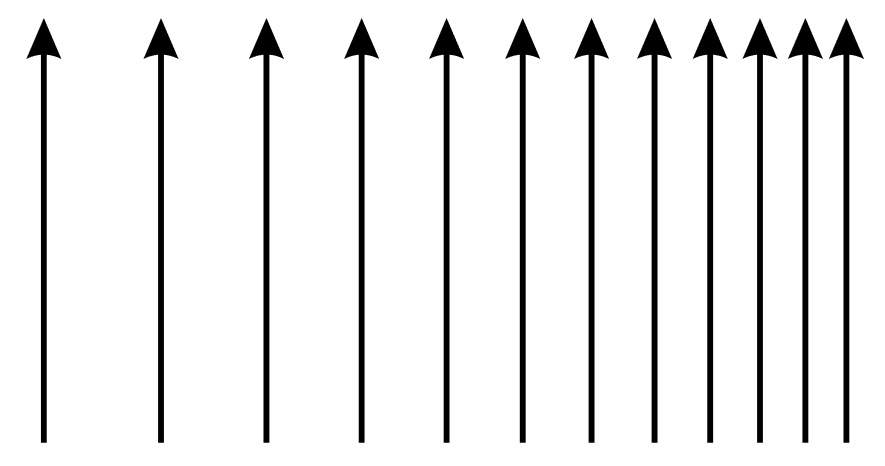
\includegraphics[width=0.5\textwidth]{S3 Figures/S3-90.png}
\end{center}
\end{solution}

\hypertarget{P91}{}
\begin{solution}{normal} % 91
Show that the potential inside a uniformly charged sphere is constant and equal to the potential of the sphere itself.
\end{solution}

\hypertarget{P92}{}
\begin{solution}{normal} % 92
a) Show that the capacitance of a parallel plate capacitor (in a vacuum) is given by the formula $\varepsilon_0 S/d$, where $S$ is the area of of the plates and $d$ is their distance of separation. b) Assuming that the electric field between the plates is $E$, show that the energy density of the capacitor is $\varepsilon_0 E^2/2$.
\end{solution}

\hypertarget{P93}{}
\begin{solution}{normal} % 93
$N$ identical droplets of mercury are charged to the same potential  $\varphi_0$. Determine the potential of a large drop of mercury when the $N$ smaller droplets coalesce (assume all the droplets are spherical).
\end{solution}

\hypertarget{P94}{}
\begin{solution}{normal} % 94
Show that the electric potential due to a dipole $\textbf{\textit{p}}$ can be expressed as $\varphi(r)=\textbf{\textit{p}}\hat{\textbf{\textit{r}}}/(4\pi\varepsilon_0r^2)$.
\end{solution}

\hypertarget{P95}{}
\begin{solution}{normal} % 95
A capacitor is formed from two concentric metal spheres, and the space between them is filled with air. If the radius of the outer sphere is $0.5\;\text{m}$ and if the air breaks down under an electric field of $30\;\text{kV}/\text{cm}$, what must the radius of the inner sphere be in order to create the highest possible potential difference? Also calculate that potential difference.
\end{solution}

\hypertarget{P96}{}
\begin{solution}{normal} % 96
Determine the strength of the electric field a distance $x$ along the axis of a ring of radius $R$ with charge $Q$ distributed evenly over its surface.
\end{solution}

\hypertarget{P97}{}
\begin{solution}{normal} % 97
Determine the radius of an electron assuming that the mass of an electron ($m_e=9.1\times10^{-31}\;\text{kg}$) is due to the electrostatic energy of its charge ($\Pi=mc^2$). In our simple model, you may assume that the charge of the electron ($e=-1.6\times10^{-19}\;\text{C}$) is evenly distributed over its "surface". 
\end{solution}

\hypertarget{P98}{}
\begin{solution}{normal} % 98
Two metal spheres with radii $R_1$ and $R_2$ are spaced a very far distance apart. If both spheres initially have charge $q$, what will the charges on the spheres be once they are connected by a wire?
\end{solution}

\hypertarget{P99}{}
\begin{solution}{normal} % 99
A point charge $q$ is placed a distance $h$ above an infinite planar conductor. Determine the surface charge density $\sigma$ induced on the surface of the conductor.
\end{solution}

\hypertarget{P100}{}
\begin{solution}{normal} % 100
A metal sphere with radius $r$ is given charge $q$. The sphere is connected to the ground with a long wire of resistance $R$. Determine the initial current through the wire.
\end{solution}

\hypertarget{P101}{}
\begin{solution}{normal} % 101
A metal sphere of radius $r$ is located inside a larger metal sphere of radius $R$. The two spheres are concentric, and the smaller sphere is grounded by a long wire (that passes through a small opening on the surface of the larger sphere). The larger sphere has no contact with the other sphere or the grounding wire. a) The outer sphere is given a charge $Q$. What charge is induced on the smaller sphere as a result? b) Determine the capacitance of the spheres.
\end{solution}

\hypertarget{P102}{}
\begin{solution}{normal} % 102
A point charge $q$ is located a distance $r$ from the center of a metal sphere of radius $R$. What is the potential of the sphere?
\end{solution}

\hypertarget{P103}{}
\begin{solution}{normal} % 103
A point charge $q$ is at a distance $h$ above the surface of a conductor in the shape of an infinite plane. What is the force acting on this point charge?
\end{solution}

\hypertarget{P104}{}
\begin{solution}{normal} % 104
A metal sphere of radius $R$ is placed in a homogeneous electric field $\textbf{\textit{E}}_0$. Determine the charge density on the surface of the sphere and the electric field in the space around the sphere. \textit{Note:} The field outside the sphere due to the surface charge density is similar to the field caused by a dipole placed at the center of the sphere (see P94).
\end{solution}

\hypertarget{P105}{}
\begin{solution}{normal} % 105 ? can't translate note
A metal cylinder of radius $R$ is placed in a homogeneous electric field $\textbf{\textit{E}}_0$ with its axis perpendicular to the field. Determine the charge density induced on the surface of the cylinder and the electric field in the space around the cylinder.
\end{solution}

\hypertarget{P106}{}
\begin{solution}{normal} % 106
A charge $q$ is located at a distance $h$ from the center of a grounded metal sphere of radius $R$. Find the force acting on the charge.
\end{solution}

\hypertarget{P107}{}
\begin{solution}{normal} % 107
Solve the previous problem if the sphere is not grounded. \textit{Tip:} The solution to P106 only needs to be slightly improved.
\end{solution}

\hypertarget{P108}{}
\begin{solution}{normal} % 108
The two plates in a parallel plate capacitor each have area $S$ and are separated by a distance $d$. Both plates are grounded. A point charge $q$ is placed between the two plates at a distance $x$ from the first plate. How much charge accumulates on each plate?
\end{solution}

\hypertarget{P109}{}
\begin{solution}{normal} % 109 ? unsure about translation
A dielectric with dielectric constant $\kappa$ is inserted between the plates of a parallel plate capacitor with area $S$ and separation $d$. a) Find the capacitance of the capacitor; b) Find the force acting between the plates of the capacitor when a potential difference of $U$ is applied across the plates 
\end{solution}

\hypertarget{P110}{}
\begin{solution}{normal} % 110
A parallel plate capacitor is immersed in a non-conductive fluid with dielectric constant $\kappa$. Determine the force between the plates if the area of the plates is $S$, their separation is $d$, and the charges on them are $\pm Q$.
\end{solution}

\hypertarget{P111}{}
\begin{solution}{normal} % 111
A dielectric slab with uniform thickness and dielectric constant $\kappa$ is placed in a homogeneous electric field $\textbf{\textit{E}}_0$, with which the plate forms an angle $\theta$. Determine the electric field inside the plate and the charge density on the surface of the plate.
\end{solution}

\hypertarget{P112}{}
\begin{solution}{normal} % 112
An infinitely long dielectric cylinder with dielectric constant $\kappa$ is placed in a homogeneous electric field $\textbf{\textit{E}}_0$. Determine the electric field inside the cylinder if the axis of the cylinder: a) is parallel to $\textbf{\textit{E}}_0$; b) lies across $\textbf{\textit{E}}_0$.
\end{solution}

\hypertarget{P113}{}
\begin{solution}{normal} % 113
Consider a dielectric sphere of radius $R$ and dielectric constant $\kappa$. Determine the field inside the sphere and the surface charge density on the surface of the sphere.
\end{solution}

\hypertarget{P114}{}
\begin{solution}{normal} % 114
A point charge $q$ is kept at a distance $h$ from the line separating two infinite dielectric planes. The dielectric constants of the planes are $\kappa_1$ and $\kappa_2$ respectively. Find the electric field in each dielectric.
\end{solution}

\hypertarget{P115}{}
\begin{solution}{normal} % 115
Determine the force acting on a dielectric sphere of radius $R$ and dielectric constant $\kappa$ in an inhomogeneous electric field $\textbf{\textit{E}}(\textbf{\textit{r}})$. \textit{Note:} See problem 113 and problem 86.
\end{solution}

\newpage
\section{Magnetostatics}
\hypertarget{P116}{}
\begin{solution}{normal} % 116
Determine the magnetic field at a distance $x$ along the axis of a loop of current. The loop has radius $R$ and has a current $I$ running through it.
\end{solution}

\hypertarget{P117}{}
\begin{solution}{normal} % 117
Determine the magnetic field due to an infinite sheet of current. The current density ($\text{A}/\text{m}$) is everywhere and equal to $\alpha$.
\end{solution}

\hypertarget{P118}{}
\begin{solution}{normal} % 118
Determine the magnetic field at a distance $r$ from an infinitely long straight wire. The current in the wire is $I$.
\end{solution}

\hypertarget{P119}{}
\begin{solution}{normal} % 119
Determine the magnetic field at a distance $r$ from the axis of a cylindrical conductor if the current density over the cross-section of the conductor is uniform and equal to $J$. The radius of the cylinder is $R$.
\end{solution}

\hypertarget{P120}{}
\begin{solution}{normal} % 120
A solenoid is a thin wire that is tightly and evenly wrapped in a cylindrical manner. Consider a long solenoid with $n$ turns per unit length along its axis with a current $I$ passing through it. Such a solenoid is the magnetic analogue of a parallel plate capacitor. Show that: a) the magnetic field inside the solenoid is homogeneous and oriented in the axial direction; b) there is no magnetic field outside the solenoid, and c) the magnetic field inside the solenoid is given by $B=\mu_0nI$.
\end{solution}

\hypertarget{P121}{}
\begin{solution}{normal} % 121
The figure below depicts two different wires each with current $I$ running through it (straight branches run to infinity). In each case, determine the magnetic force at the point marked with a black dot.
\begin{center}
    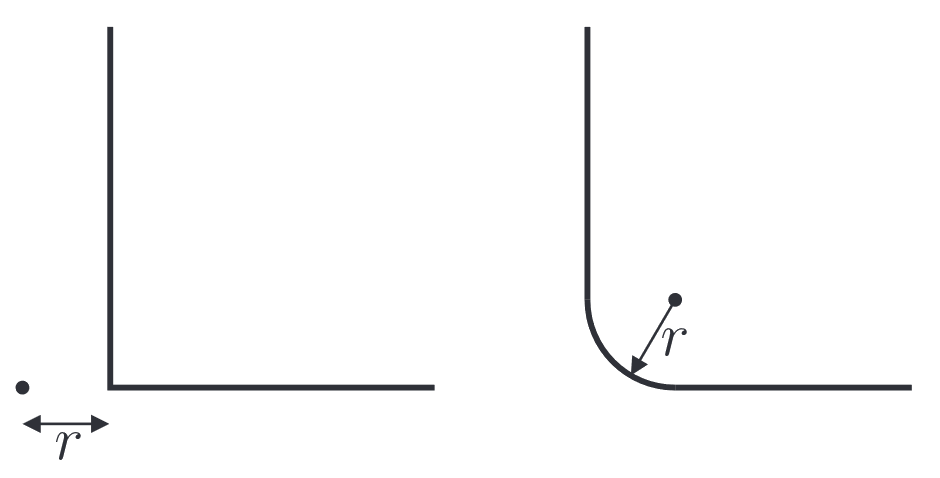
\includegraphics[width=0.5\textwidth]{S4 Figures/S4-121.png}
\end{center}
\end{solution}

\hypertarget{P122}{}
\begin{solution}{normal} % 122
Determine the magnetic field at the end of a long solenoid. A current $I$ runs through the solenoid, which has $n$ turns per unit length.
\end{solution}

\hypertarget{P123}{}
\begin{solution}{normal} % 123
Determine the magnetic field in the cavity formed by the intersection of two straight, infinitely long, cylindrical conductors as shown in the figure below. The current densities in each of the conductors are equal but in opposite directions ($\pm J$), the radius of both conductors is $R$, and the distance between their centers is $d$.
\begin{center}
    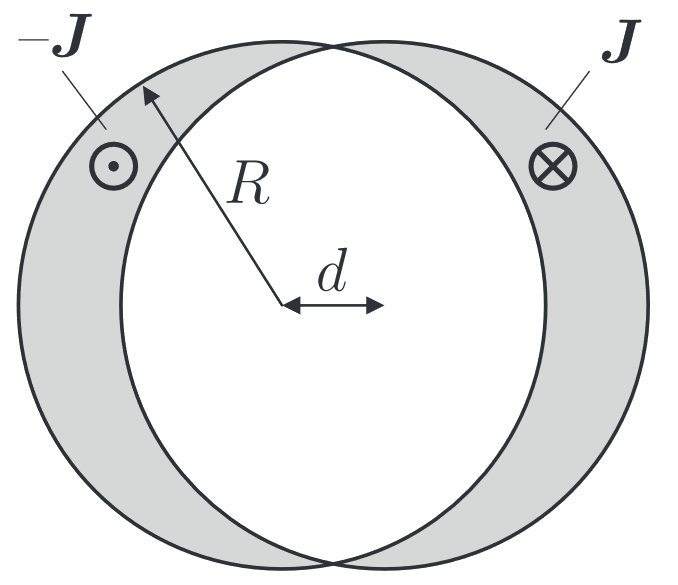
\includegraphics[width=0.35\textwidth]{S4 Figures/S4-123.png}
\end{center}
\end{solution}

\hypertarget{P124}{}
\begin{solution}{normal} % 124
Determine the force per unit length between two infinitely long straight parallel wires if the currents in the wires are $I_1$ and $I_2$ and the distance between the wires is $r$.
\end{solution}

\hypertarget{P125}{}
\begin{solution}{normal} % 125
A charge $Q$ is evenly distributed over a sphere of radius $R$. The sphere rotates at an angular velocity $\omega$ about an axis through its center. Determine the magnetic moment of such a system. \textit{Note:} Divide the surface of the sphere into infinitely thin layers and add the area of a thin spherical segment $\Delta S=2\pi R\Delta h$.
\end{solution}

\hypertarget{P126}{}
\begin{solution}{normal} % 126
A permanent magnet is hung by a thread. Its magnetic moment is $\textbf{\textit{p}}$ (which lies on a horizontal plane) and its moment of inertia from the attachment point of the thread relative to the vertical axis is $I$. Determine the oscillation period of small-amplitude oscillations when a homogeneous horizontal magnetic field $B$ is generated in space.
\end{solution}

\hypertarget{P127}{}
\begin{solution}{normal} % 127
Two permanent magnets (with magnetic moments $\textbf{\textit{p}}_1$ and $\textbf{\textit{p}}_1$) are placed a distance $r$ from each other (where $r$ is much greater than the dimensions of the magnets). Determine the force acting between the magnets.
\end{solution}

\hypertarget{P128}{}
\begin{solution}{normal} % 128
The ratio of the magnetic moment of a particle to its angular momentum is known as the gyromagnetic ratio of that particle. Find the gyromagnetic ratio for the orbital motion of an electron using the Bohr model. \textit{Note:} According to Bohr's theory, the electron orbits the nucleus in a circular orbit where the orbital momentum of the electron is quantized: $mvr=n\hbar$, where $n=1,2,3\dots$.
\end{solution}

\hypertarget{P129}{}
\begin{solution}{normal} % 129
The magnetic moment of an iron atom is given by $p=2.2\mu_B$, where $\mu_B= e\hbar/2m_e\approx9.27\times10^{-24}\;\text{A}\;\text{m}^2$ (also known as the Bohr magneton). The distance between adjacent atoms in the cubic crystal lattice of iron is $d=2.3\;\AA$. What is the maximum magnetic field that can be generated by magnetized iron in the absence of an external magnetic field?
\end{solution}

\hypertarget{P130}{}
\begin{solution}{normal} % 130
Determine the magnetic field inside an infinitely long solenoid if the solenoid is filled with a substance with relative magnetic permeability $\mu$. The ampere-turns per unit length of the solenoid is given by $nI$.
\end{solution}

\hypertarget{P131}{}
\begin{solution}{normal} % 131
A spherical magnet with relative magnetic permeability $\mu$ is placed in a homogeneous magnetic field $\textbf{\textit{B}}_0$. Determine the magnetic field inside the sphere. \textit{Tip:} the magnetic field of a uniformly magnetized sphere outside the sphere is similar to the field produced by a magnetic dipole placed in the center of the sphere.
\end{solution}

\hypertarget{P132}{}
\begin{solution}{normal} % 132
An electromagnet used in a laboratory consists of an iron core (with relative magnetic permeability $\mu$) and a wire wound around it $N$ times, as shown in the diagram below. The width $d$ of the air gap is much smaller than the thickness of the core. If the length of the core is $l$ and the current in the wire is $I$, determine the magnetic field in the air gap of the core.
\begin{center}
    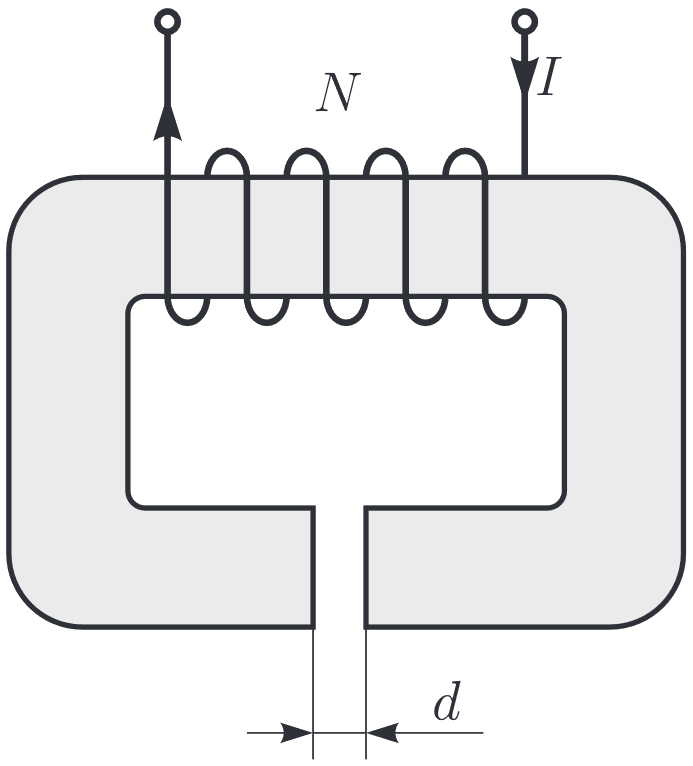
\includegraphics[width=0.6\textwidth]{S4 Figures/S4-132.png}
\end{center}
\end{solution}

\hypertarget{P133}{}
\begin{solution}{normal} % 133
The electromagnet shown below consists of a core (1) and and an anchor (2); the relative permeability of each is $\mu$. A wire is wrapped $N$ times around the core, through which a current $I$ is passed. The cross-sectional area of the core and anchor is $S$ and it has total length $l$. Find the force by which the core holds the anchor. \textit{Note:} A virtual shift method can be used here. However, note that changing the distance between the core and anchor induces an emf in the coil.
\begin{center}
    \includegraphics[width=0.6\textwidth]{S4 Figures/S4-133.png}
\end{center}
\end{solution}

\hypertarget{P134}{}
\begin{solution}{normal} % 134
Parallel to and at a distance $h$ above the surface of an infinite planar superconductor is an infinitely long straight wire with current $I$ running though it. Determine the force acting on a unit length of this wire.
\end{solution}

\newpage
\section{Electromagnetic Induction}
\hypertarget{P135}{}
\begin{solution}{normal} % 135
One method of measuring magnetic field is as follows. A small coil is inserted into the magnetic field with its axis parallel to $\textbf{\textit{B}}$. The terminals of the coil are connected to a ballistic galvanometer, which measures the amount of charge passed through it. The coil is then quickly rotated $180\degree$. How much charge passes through the galvanometer if the area of the coil is $S$, the number of turns is $N$, and the resistance of the coil is $R$?
\end{solution}

\hypertarget{P136}{}
\begin{solution}{normal} % 136
Two horizontal infinitely long parallel metal rails with negligible resistance are placed a distance $l$ from each other. The rails are connected to a capacitor of capacitance $C$ and voltage $U_0$. If there is a homogeneous vertical magnetic field of magnitude $\textbf{\textit{B}}$, a) what is the maximum velocity the rod reaches, and b) what is the maximum possible efficiency of such an "electromagnetic cannon" (i.e. how much of the energy stored in the capacitor can be converted into kinetic energy in the rod)?
\end{solution}

\hypertarget{P137}{}
\begin{solution}{normal} % 137
A dielectric ring of mass $m$ is attached by spokes of negligible mass to an axis around which it can rotate frictionlessly. A charge $Q$ is evenly distributed over the ring. Initially, the (stationary) ring is located along the axis of a homogeneous magnetic field $\textbf{\textit{B}}$. After some time, the magnetic field is switched off. What is the final angular velocity of the ring?
\end{solution}

\hypertarget{P138}{}
\begin{solution}{normal} % 138
In the circuit below, switch $K$ has been closed for a long time and all the bulbs have the same brightness. For each of the bulbs, how many times does the current through the bulb change immediately after opening switch $K$.
\begin{center}
    \includegraphics[width=0.8\textwidth]{S5 Figures/S5-138.png}
\end{center}
\end{solution}
\newpage
\hypertarget{P139}{}
\begin{solution}{normal} % 139
In the circuit shown below, switch $K$ has been open for a long time. a) What is the ammeter reading immediately after closing the switch? b) The switch is kept closed until the current reaches a steady state. What is the ammeter reading now? c) After the current has reached a steady state, what is the ammeter reading immediately after opening the switch?
\begin{center}
    \includegraphics[width=0.4\textwidth]{S5 Figures/S5-139.png}
\end{center}
\end{solution}

\hypertarget{P140}{}
\begin{solution}{normal} % 140
Circuit element $E$ with $I-V$ dependence as shown in the graph below is connected to a circuit an inductor and battery. How does the voltage on element $E$ change over time? Determine time steps.
\begin{center}
    \includegraphics[width=0.8\textwidth]{S5 Figures/S5-140.png}
\end{center}
\end{solution}

\hypertarget{P141}{}
\begin{solution}{normal} % 141
A battery with emf $\mathcal{E}=12\;\text{V}$ is charged by a DC voltage source as shown in the figure below. The inductance in the coil is $L=1\;\text{H}$ and it has negligible resistance. The diode can be assumed to be ideal. Switch $K$ closes and opens periodically, alternating from being closed for time $\tau_1$ to being open for time $\tau_2$, where $\tau_1=\tau_2=0.01\;\text{s}$. Determine the average charging current.
\begin{center}
    \includegraphics[width=0.45\textwidth]{S5 Figures/S5-141.png}
\end{center}
\end{solution}

\hypertarget{P142}{}
\begin{solution}{normal} % 142
Determine the inductance of a solenoid if its diameter is much smaller than its length $l$. The number of turns is $N$ and the cross-sectional area of the solenoid is $S$. The solenoid is wound around a ferromagnetic core with relative magnetic permeability $\mu$.
\end{solution}

\hypertarget{P143}{}
\begin{solution}{normal} % 143
Assuming that the work done to generate current in a solenoid $LI^2/2$ goes into the energy of its magnetic field, show that the energy density of the magnetic field is given by $B^2/2\mu_0$.
\end{solution}

\hypertarget{P144}{}
\begin{solution}{normal} % 144
Determine the inductance of a straight wire of length $l$ and radius $a$.
\end{solution}

\hypertarget{P145}{}
\begin{solution}{normal} % 145
Show that the mutual inductances $L_{12}$ and $L_{21}$ are always equal. \textit{Note:} Find the energy of the coupled circuits if the currents $I_1$ and $I_2$ flow through them. To do this, calculate the work the current sources need to do in order to generate the currents and show that the result is unambiguous only under the condition $L_{12}=L_{21}$.
\end{solution}

\hypertarget{P146}{}
\begin{solution}{normal} % 146
Show that $M\leq\sqrt{L_1L_2}$, where $M$ is the mutual inductance and $L_1,L_2$ are the self-inductances of the coupled circuits. \textit{Note:} Show that for $M>\sqrt{L_1L_2}$, conservation of energy is violated, namely that increasing the current in one of the circuits induces an emf in the circuit, which causes the current to increase further ($\mathcal{E}_1dI_1>0$).
\end{solution}

\hypertarget{P147}{}
\begin{solution}{normal} % 147
A toroid consists of a thin wire wrapped around a torus. Let the major and minor radii of the toroid be $R$ and $r$, respectively, where $r\ll R$ and let the number of turns of the wire be $N$. Determine the mutual inductance between the toroid and a straight wire. Prove that the equation $L_{12}=L_{21}$ is valid for this system.
\end{solution}

\hypertarget{P148}{}
\begin{solution}{normal} % 148
Determine the mutual inductance between two coils wrapped around a common toroidal core. The first coil has $N_1$ turns and the second has $N_2$ turns. The length of the core is $l$ and has cross-sectional area $S$ and relative magnetic permeability $\mu$.
\end{solution}

\hypertarget{P149}{}
\begin{solution}{normal} % 149
Two coils are wound around a common ferromagnetic core. The first has $N_1$ turns and the second $N_2$ turns, where $N_1/N_2=n$. The coils have negligible resistance. The ends of the second coil are connected to resistor $R$, and a DC voltage source of voltage $U$ is connected to the terminals of the first coil. Show that the power dissipated by the resistor is given by $n^2U^2/R$.
\end{solution}

\hypertarget{P150}{}
\begin{solution}{normal} % 150
A capacitor with capacitance $C$ is charged with an inductor and a diode from a constant voltage source $\mathcal{E}$. The internal resistance of the voltage source and the resistance of the coils are negligible. a) What was the voltage across the capacitor at the beginning when the charge on the capacitor was zero? b) What is the maximum current in the circuit? The $I-V$ graph of the diode is given in the graph below.
\begin{center}
    \includegraphics[width=0.4\textwidth]{S1 Figures/S1-35-2.png}
\end{center}
\end{solution}

\hypertarget{P151}{}
\begin{solution}{normal} % 151
In the circuit shown below, capacitors $C_1$ and $C_2$ are charged by a DC voltage source of emf $\mathcal{E}$. Switch $K$ is now closed. What is a) the maximum current $I_\text{max}$ through the coil, and b) the maximum voltage $U_\text{max}$ on capacitor $C_1$ achieved after closing the switch? \textit{Note:} To answer part b, note that if capacitor $C_1$ has maximal voltage across it then $C_2$ has minimal voltage across it as the sum of these voltages are constant (and equal to $\mathcal{E}$).
\begin{center}
    \includegraphics[width=0.35\textwidth]{S5 Figures/S5-151.png}
\end{center}
\end{solution}

\newpage
\section{AC Circuits}
\hypertarget{P152}{}
\begin{solution}{normal} % 152
A heater with power $30\;\text{W}$ is designed for a mains voltage of $220\;\text{V}$. How large of a capacitor should be connected in series with the heater to reduce its power to $20\;\text{W}$? Do not consider the temperature-dependence of the heater's resistance into account.
\end{solution}

\hypertarget{P153}{}
\begin{solution}{normal} % 153
[IPhO 1982] A fluorescent lamp is connected to a mains electricity supply as shown in the figure below. The mains frequency is $50\;\text{Hz}$ and supplies an emf of $228.5\;\text{V}$. The current in the circuit is $0.60\;\text{A}$, the voltage across the lamp is $84\;\text{V}$, and the resistance in the coil is $26.3\;\Omega$. Assume that the fluorescent lamp is ohmic. Starter $S$ is a switch that closes when the lamp is switched on, but quickly opens again and remains open when the lamp is lit. a) What is the inductance $L$ of the coil? b) Determine the phase shift $\Delta\phi$ between the voltage and the current. c) What power $P$ is dissipated by the circuit? d) It is sometimes necessary to compensate for the reactive current resulting from the simultaneous use of many fluorescent lamps (see P154). A capacitor of what capacitance should be connected in series with the coil in order to reverse the phase shift? (Kalda Circuits P87)
\begin{center}
    \includegraphics[width=0.65\textwidth]{S6 Figures/S6-153.png}
\end{center}
\end{solution}

\hypertarget{P154}{}
\begin{solution}{normal} % 154 ? actually have no idea what this is about
A cottage receives power from a substation via a long single-phase overhead power line. As a result, in addition to an electric meter, the house has a voltmeter to check the voltage reaching the house. After returning the the cottage after a three month absence, you discover that although all your appliances (including your lights) have been switched off, the transformer you were using had been consuming power. However, this energy consumption was not shown on your electric meter, and you want to determine how many kilowatt-hours of energy you didn't pay Eesti Energia for heating the air with an overhead line. To do this, you took three separate voltage readings: (1) $U_t=234.0\;\text{V}$ if only the transformer is connected to the mains; (2) $U_0=236.0\;\text{V}$ if everything (including the transformer) is switched off; and (3) $U_r=219.6\;\text{V}$ if the transformer is off but the electric radiator is on. You also determined, for the third case, that the power consumption of the radiator was $P_r=1200\;\text{W}$. Similarly, you recorded that if only the transformer is switched on, it consumes power $P_t=5\;\text{W}$. How many kilowatt-hours of energy did the transformer/overhead line consume during your absence?
\end{solution}

\hypertarget{P155}{}
\begin{solution}{normal} % 155
The figure below is also known as a Maxwell bridge, a circuit used to determine the inductance $L$ and resistance $R$ of the inductor. To do this, resistors $R_1,R_2,R_C$ and capacitor $C$ are adjusted until the voltmeter $V$ reads $0$. Determine $L$ and $R$ in terms of $R_1,R_2,R_C$, and $C$.
\begin{center}
    \includegraphics[width=0.5\textwidth]{S6 Figures/S6-155.png}
\end{center}
\end{solution}

\hypertarget{P156}{}
\begin{solution}{normal} % 156
The figure below shows a circuit that can be used to change the phase of an alternating signal. Show that, for a negligible output current, the output voltage is the same as the input voltage, but with a phase shift of $2\arctan(\omega RC)$ (or $2\arctan(-1/\omega RC)$). (Kalda Circuits P95)
\begin{center}
    \includegraphics[width=0.45\textwidth]{S6 Figures/S6-156.png}
\end{center}
\end{solution}
\newpage
\hypertarget{P157}{}
\begin{solution}{normal} % 157
The circuit in the figure below is supplied with an AC voltage source with RMS voltage $U$. Determine the power dissipated in the circuit. \textit{Note:} The power dissipated can be found in two ways: by summing the individual powers $I^2R$ on all resistors or by using formula 9 for the whole circuit.
\begin{center}
    \includegraphics[width=0.35\textwidth]{S6 Figures/S6-157.png}
\end{center}
\end{solution}

\hypertarget{P158}{}
\begin{solution}{normal} % 158
The relationship between the voltages and currents of the primary and secondary coils of a transformer are generally very complex. However, real transformers are often close to an ideal transformer, which has the following properties: 1) The inductances $L_1$ and $L_2$ of the coils are very high; 2) The coupling between the primary and secondary coils is maximal; 3) The resistances of the coils are negligible; and 4) Losses in the core (hysteresis, eddy currents, etc.) are negligible. Show that in this case all currents and voltages have the same phase and the following equations hold:
$$\dfrac{U_2}{U_1}=n,\;\;\;\;\dfrac{I_2}{I_1}=\dfrac{1}{n},$$
where $n$ is the ratio between the number of turns in the secondary coil to the number of turns in the primary coil.
\end{solution}

\hypertarget{P159}{}
\begin{solution}{normal} % 159
In the LC circuit shown below, $L_1=10\;\text{mH}$, $L_2=20\;\text{mH}$, $C_1=10\;\text{nF}$, and $C_2=5\;\text{nF}$. At some point in time, the current through $L_1$ was equal to $I_1=0.1\;\text{A}$ and the voltage across $C_1$ at the same time was $U_0=40\;\text{V}$. What is the amplitude of current oscillations in coil $L_2$?
\begin{center}
    \includegraphics[width=0.22\textwidth]{S6 Figures/S6-159.png}
\end{center}
\end{solution}

\hypertarget{P160}{}
\begin{solution}{normal} % 160
Determine the natural oscillation frequency of the LC circuit shown below.
\begin{center}
    \includegraphics[width=0.4\textwidth]{S6 Figures/S6-160.png}
\end{center}
\end{solution}

\hypertarget{P161}{}
\begin{solution}{normal} % 161
Determine the natural oscillation frequencies of the LC circuit shown below. \textit{Note:} The equation $a^2=b^2$ satisfies both $a=b$ and $a=-b$. (Kalda Circuits P99)
\begin{center}
    \includegraphics[width=0.4\textwidth]{S6 Figures/S6-161.png}
\end{center}
\end{solution}

\newpage
\section{Movement of Charged Particles in Electric and Magnetic Fields}
\hypertarget{P162}{}
\begin{solution}{normal} % 162
An electron with velocity $v$ moves in a homogeneous magnetic field $\textbf{\textit{B}}$, where $\textbf{\textit{v}}\bot \textbf{\textit{B}}$. Determine the radius of the electron's trajectory.
\end{solution}

\hypertarget{P163}{}
\begin{solution}{normal} % 163
A beam of electrons is emitted from a point source. The magnitudes of the velocities $v$ of the electrons are equal, but they are scattered by an angle of up to $\alpha$ with respect to the direction of the homogeneous magnetic field $B$ in the space, where $\alpha\ll 1$. At what distance from the point source does the electron beam focus again?
\end{solution}

\hypertarget{P164}{}
\begin{solution}{normal} % 164
Two parallel electrodes (a cathode and an anode) are located a distance $d$ from each other in a vacuum. A positive potential $U$ is applied from the cathode to the anode. From the surface of the cathode, an electron with initial velocity zero is accelerated by the electric field. How strong of a magnetic field $\textbf{\textit{B}}$ perpendicular to the electric field must be generated between the electrodes so that the electron no longer reaches the anode?
\end{solution}

\hypertarget{P165}{}
\begin{solution}{normal} % 165
Two coaxial cylindrical conductors are located in a vacuum. The inner (cathode) radius is $a$ and the outer (anode) radius is $b$. The anode is given a positive potential $U$ with respect to the cathode. There is a homogeneous magnetic field $\textbf{\textit{B}}$ in the space between the cylinders. An electron begins to move with initial speed zero from the surface of the cathode due to the electric field. Determine the critical value of $\textbf{\textit{B}}$ for which the electron no longer reaches the anode.
\end{solution}

\hypertarget{P166}{}
\begin{solution}{normal} % 166
An electron with initial velocity $v_0$ travels in a homogeneous electric and magnetic field. The vectors $v_0,\textbf{\textit{E}}$, and $\textbf{\textit{B}}$ are all perpendicular to each other and $v_0=\textbf{\textit{B}}\times\textbf{\textit{E}}$. What is the trajectory of the electron? What is its average speed $\left<v\right>$? Assume that $E/B\ll c$ and $v\ll c$.
\end{solution}

\hypertarget{P167}{}
\begin{solution}{normal} % 167
In metals, each atom donates, on average, one valence electron. Determine the drift velocity of electrons in copper wire with current density $5\;\text{A}/\text{mm}^2$. The density of copper is $8900\;\text{kg}/\text{m}^3$ and its molar mass is $63.5\;\text{g}/\text{mol}$.
\end{solution}

\hypertarget{P168}{}
\begin{solution}{normal} % 168
Two identical metal spheres of radius $r$ are placed in a homogeneous conductive medium with resistivity $\rho$. The distance between the spheres is much larger than their radius. What is the resistance between the spheres?
\end{solution}

\hypertarget{P169}{}
\begin{solution}{normal} % 169
One problem in determining the resistivity $\rho$ of a semiconductor is the unknown voltage drop across the contacts. This problem can be solved with the following method, which we analyze here using a semi-infinite thin plate (with thickness $h$) for simplicity. Let the four contacts be soldered to the edge of the plate as shown in the diagram below. a) Current I passes though contacts $A$ and $B$. Show that a voltmeter connected between contacts $C$ and $D$ measures a voltage of
$$U=\dfrac{I\rho}{\pi h}\ln\left(\dfrac{(a+b+c)b}{(a+b)(b+c)}\right).$$
Let the ratio $U/I$ be $R_{AB,CD}$. b) Show analogously that when current $I$ passes through contacts $B$ and $C$, then
$$R_{BC,AD}=\dfrac{\rho}{\pi h}\ln\left(\dfrac{(a+b)}{(b+c)}{ac}\right)$$
c) Show that
$$\exp(\pi hR_{AB,CD}/\rho)+\exp(\pi hR_{BC,AD}/\rho)=1$$
The obtained relationship allows us to determine $\rho$ after measuring $R_{AB,CD}$ and $R_{BC,AD}$.
\begin{center}
    \includegraphics[width=0.4\textwidth]{S7 Figures/S7-169.png}
\end{center}
\blfootnote{It is not specified what $a$, $b$, and $c$ are, but it is likely that $a=AB$, $b=BC$, and $c=CD$}
\end{solution}

\hypertarget{P170}{}
\begin{solution}{normal} % 170
With the method described below, it is possible to measure the resistivity of a material without attaching contacts to the material. A disk-shaped piece of material is placed in a homogeneous magnetic field generated inside a solenoid so that the axis of the disk is parallel to the axis of the solenoid. The solenoid is supplied by an AC source with frequency $\omega$ such that $B(t)=B_0\cos(\omega t)$. The disk has radius $R$ and thickness $d$. Determine the resistivity of the disk if the disk dissipates power $P$. \textit{Note:} You may need the formula $\left<\sin^2\alpha\right>=\left<\cos^2\alpha\right>=1/2$ and the integral $\int x^ndx=x^{n+1}/(n+1)$.
\end{solution}

\hypertarget{P171}{}
\begin{solution}{normal} % 171
A metal plate is located in a homogeneous magnetic field $\textbf{\textit{B}}$ that is perpendicular to the surface of the plate. Determine the drag force caused by the eddy currents in the plate as the plate moves at a speed $\textbf{\textit{v}}$ perpendicular to $\textbf{\textit{B}}$. The area of the plate is $S$, its thickness is $d$, and it has resistivity $\rho$. \textit{Note:} There are several ways to get an approximate answer. One possibility is to use conservation of energy by estimating the heat generated in the plate due to the eddy currents.
\end{solution}
\newpage
\hypertarget{P172}{}
\begin{solution}{normal} % 172
Determine the strength of the transverse electric field due to the Hall effect for the situation shown in the image below. Assume that there is only one type of charge carrier in the material, with charge $q$ and charge carrier density $n$.
\begin{center}
    \includegraphics[width=0.5\textwidth]{S7 Figures/S7-172.png}
\end{center}
\end{solution}

\hypertarget{P173}{}
\begin{solution}{normal} % 173
A semiconductor that measures the strength of a magnetic field using the Hall effect is called a Hall sensor. Construct a circuit diagram for a wattmeter if a Hall sensor, solenoid, and voltmeter are used.
\end{solution}

\hypertarget{P174}{}
\begin{solution}{normal} % 174
An electromagnetic pump can be used to pump liquids with good electrical conductivity (a schematic is shown in the figure below). A liquid with resistivity $\rho$ moves at speed $v$ through the pump. The vectors $\textbf{\textit{v}},\textbf{\textit{B}}$, and $\textbf{\textit{E}}$ are all mutually perpendicular. a) Show that the fluid is subjected to a force $\textbf{\textit{F}}=B^2(\textbf{\textit{u}}-\textbf{\textit{v}})/\rho$, where $\textbf{\textit{u}}=\textbf{\textit{E}}\times\textbf{\textit{B}}/B^2$. b) Show that the maximum efficiency of the pump is $0.5$. Assume that the magnetic field creates a permanent magnet and that edge effects are negligible. 
\begin{center}
    \includegraphics[width=0.5\textwidth]{S7 Figures/S7-174.png}
\end{center}
\end{solution}

\hypertarget{P175}{}
\begin{solution}{normal} % 175
A homopolar motor consists of a copper disk attached to a shaft that rotates in a homogeneous magnetic field $\textbf{\textit{B}}$ directed parallel to the axis of the disk. Current flows into the disk through the shaft and exits through the side of the disk. The radius of the shaft is $a$, the radius of the disk $b$, and the thickness of the disk $h$. The resistivity of the disk is $\rho$. a) Determine the torque $M$ exerted on the disk by the magnetic field when a current $I$ flows through it. b) Determine the heat $P$ dissipated by the disk when a current $I$ flows through it. c) Find the potential difference $U$ between the axis and the edge of the disk when it is rotating at an angular velocity $\omega$. d) Show that conservation of energy holds in the form $VI=M\omega+P$. \textit{Note:} The problems requires taking a few simple integrals: $\int xdx=x^2/2,\int (1/x)dx=\ln x$.
\end{solution}

\newpage
\section{Answers}
\begin{multicols}{2}
\begin{enumerate}
	\item [\hyperlink{P1}{1}.] $I_1=1.5\;\text{A};\;I_2=1.7\;\text{A}$ % 1
	\item [\hyperlink{P2}{2}.]  % 2
	\item [\hyperlink{P3}{3}.]  % 3
	\item [\hyperlink{P4}{4}.] Increases $\approx$ 1.14 times % 4
	\item [\hyperlink{P5}{5}.] $R=(2/9)R_0$ % 5
	\item [\hyperlink{P6}{6}.] $\rho\approx24\;\Omega\;\text{m}$ % 6
	\item [\hyperlink{P7}{7}.] $R\approx14\;\Omega$ % 7
	\item [\hyperlink{P8}{8}.] $900\;\Omega$ % 8
	\item [\hyperlink{P9}{9}.] $12\;\text{V}$ % 9
	\item [\hyperlink{P10}{10}.] $26/7\;\Omega$ % 10
	\item [\hyperlink{P11}{11}.] $I=0.5\;\text{A}$ % 11
	\item [\hyperlink{P12}{12}.]  % 12
	\item [\hyperlink{P13}{13}.]  % 13
	\item [\hyperlink{P14}{14}.] $I_4=3\;\text{A},\;I_3=2\;\text{A}$ % 14
	\item [\hyperlink{P15}{15}.]  % 15
	\item [\hyperlink{P16}{16}.] $R=1\;\Omega$ % 16
	\item [\hyperlink{P17}{17}.] Proof % 17
	\item [\hyperlink{P18}{18}.]  % 18
	\item [\hyperlink{P19}{19}.]  % 19
	\item [\hyperlink{P20}{20}.]  % 20
	\item [\hyperlink{P21}{21}.] $$\mathcal{E}=\dfrac{\sum_i\left(\dfrac{\mathcal{E}_i}{r_i}\right)}{\sum_i\left(\dfrac{1}{r_i}\right)},\;\;\;r=\left(\sum_i\dfrac{1}{r_I}\right)^{-1}$$ % 21
	\item [\hyperlink{P22}{22}.] Same as P21 % 22
	\item [\hyperlink{P23}{23}.]  % 23
	\item [\hyperlink{P24}{24}.] $R=11/6\;\Omega$ % 24
	\item [\hyperlink{P25}{25}.]  % 25
	\item [\hyperlink{P26}{26}.] $R=1\;\Omega$ % 26
	\item [\hyperlink{P27}{27}.] $4\;\text{A}$ % 27
	\item [\hyperlink{P28}{28}.] $1\;\text{mA},\;4\text{V}$ % 28
	\item [\hyperlink{P29}{29}.] $R=\frac{R_1}{2}\left(1+\sqrt{1+4R_2/R_1}\right)$ % 29
	\item [\hyperlink{P30}{30}.] $r'=\frac{R}{2}\left(1+\sqrt{1+4R/r}\right),\;\mathcal{E}'=\mathcal{E}$ % 30
	\item [\hyperlink{P31}{31}.] $R=1/3\;\Omega$ % 31
	\item [\hyperlink{P32}{32}.] $R=1/3\;\Omega$ % 32
	\item [\hyperlink{P33}{33}.] $R=1/2\;\Omega$ % 33
	\item [\hyperlink{P34}{34}.]  % 34
	\item [\hyperlink{P35}{35}.] $0.75\;\text{mW},\;0\;\text{W},\;0\;\text{W}$ % 35
	\item [\hyperlink{P36}{36}.] $I\approx8\;\text{mA}$ % 36
	\item [\hyperlink{P37}{37}.]  % 37
	\item [\hyperlink{P38}{38}.] $P\approx0.48\;\text{W}$ % 38
	\item [\hyperlink{P39}{39}.] $U_0\approx U_1+I_1R$ % 39
	\item [\hyperlink{P40}{40}.] $\sim 3$ times % 40
	\item [\hyperlink{P41}{41}.] $I=2.97\;\text{mA}$ % 41
	\item [\hyperlink{P42}{42}.] Proof % 42
	\item [\hyperlink{P43}{43}.] $l\approx12\;\text{cm},\;d\approx5.8\;\mu\text{m},\;T\approx2650\;\text{K}$ % 43
	\item [\hyperlink{P44}{44}.]  % 44
	\item [\hyperlink{P45}{45}.]  % 45
	\item [\hyperlink{P46}{46}.] $Q=C\mathcal{E}^2/2$ % 46
	\item [\hyperlink{P47}{47}.] $Q\approx123\;\mu\text{J}$ % 47
	\item [\hyperlink{P48}{48}.] Proof % 48
	\item [\hyperlink{P49}{49}.] $Q=2C\mathcal{E}^2/27$ % 49
	\item [\hyperlink{P50}{50}.]  % 50
	\item [\hyperlink{P51}{51}.] $F\approx6.4\;\mu\text{N}$ % 51
	\item [\hyperlink{P52}{52}.] $M=\varepsilon_0R^2U^2/(4d)$ % 52
	\item [\hyperlink{P53}{53}.] $F=(\kappa-1)\varepsilon_0aU^2/(2d)$ % 53
	\item [\hyperlink{P54}{54}.] $h=(\kappa-1)\varepsilon_0U^2/(2d^2\rho g)$ % 54
	\item [\hyperlink{P55}{55}.] $\tau\sim 50\;\text{s}$ % 55
	\item [\hyperlink{P56}{56}.] $t=20\;\text{s}$ % 56
	\item [\hyperlink{P57}{57}.] $\tau=\left(R_1+\dfrac{R_2R_3}{R_2+R_3}\right)C$ % 57
	\item [\hyperlink{P58}{58}.] a) $P=(U_2-U_1)^2/(4R)$
	
	b) $P=C(U_2-U_1)^2/T$ % 58
	\item [\hyperlink{P59}{59}.] a) $(I_2-I_1)T/(8C)$
	
	b) $(I_2-I_1)R/2$ % 59
	\item [\hyperlink{P60}{60}.] a) $8\;\text{k}\Omega$ and $3.2\;\text{W}$
	
	b) $50\;\mu\text{F}$ % 60
	\item [\hyperlink{P61}{61}.] $F=(1+2\sqrt{2})q^2/(8\pi\varepsilon_0 L^2)$ % 61
	\item [\hyperlink{P62}{62}.] $15:30$ (either the ans is off or my translation is off) % 62
	\item [\hyperlink{P63}{63}.]  % 63
	\item [\hyperlink{P64}{64}.]  % 64
	\item [\hyperlink{P65}{65}.]  % 65
	\item [\hyperlink{P66}{66}.] Proof % 66
	\item [\hyperlink{P67}{67}.] $E=\sigma/(2\varepsilon_0)$ % 67
	\item [\hyperlink{P68}{68}.] Between the plates: $E=\sigma/\varepsilon_0$
	
	Outside: $E=0$; $p=\sigma^2/(2\varepsilon_0)$ % 68
	\item [\hyperlink{P69}{69}.] $\rho\approx4.4\times10^{-12}\;\text{C}/\text{m}^3$ % 69
	\item [\hyperlink{P70}{70}.] $E=\lambda/(2\pi\varepsilon_0r)$ % 70
	\item [\hyperlink{P71}{71}.] Proof % 71
	\item [\hyperlink{P72}{72}.] $E(r)=\rho r/(3\varepsilon_0)$ if $r<R$
	
	$E(r)=\rho R^3/(3\varepsilon_0r^2)$ if $r\geq R$ % 72
	\item [\hyperlink{P73}{73}.] $E(r)=\rho r/(2\varepsilon_0)$ if $r<R$
	
	$E(r)=\rho R^2/(2\varepsilon_0r)$ if $r\geq R$ % 73
	\item [\hyperlink{P74}{74}.] Proof % 74
	\item [\hyperlink{P75}{75}.] a) $\textbf{\textit{E}}=\rho\textbf{\textit{d}}/(3\varepsilon_0)$
	
	b) $\textbf{\textit{E}}=\rho\textbf{\textit{d}}/(2\varepsilon_0)$ (homogeneous field) % 75
	\item [\hyperlink{P76}{76}.] $\textbf{\textit{E}}(\textbf{\textit{r}})=\rho\textbf{\textit{r}}_0/(3\varepsilon_0)$ (homogeneous field) % 76
	\item [\hyperlink{P77}{77}.] Proof % 77
	\item [\hyperlink{P78}{78}.] $F=Q\lambda/(2\pi\varepsilon_0 r)$ % 78
	\item [\hyperlink{P79}{79}.] $p=\sigma^2/(2\varepsilon_0)$ % 79
	\item [\hyperlink{P80}{80}.] $F=Q^2/(32\varepsilon_0R^2)$ % 80
	\item [\hyperlink{P81}{81}.] $\textbf{\textit{E}}_{\parallel}(r)=2\textbf{\textit{p}}/(4\pi\varepsilon_0r^3)$
	
	$\textbf{\textit{E}}\bot(r)=-\textbf{\textit{p}}/(4\pi\varepsilon_0r^3)$ % 81
	\item [\hyperlink{P82}{82}.] Proof % 82
	\item [\hyperlink{P83}{83}.] $E=SU/(4\pi r^3)$ % 83
	\item [\hyperlink{P84}{84}.] $\textbf{\textit{M}}=\textbf{\textit{p}}\times\textbf{\textit{E}}$ % 84
	\item [\hyperlink{P85}{85}.] $\Pi=-\textbf{\textit{pE}}$ % 85
	\item [\hyperlink{P86}{86}.]  % 86
	\item [\hyperlink{P87}{87}.]  % 87
	\item [\hyperlink{P88}{88}.] $\nu\sim\dfrac{1}{\pi}\sqrt{\dfrac{qE}{2ml}}\approx1.5\times10^{10}\;\text{Hz}$ % 88
	\item [\hyperlink{P89}{89}.] $v_0=d\sqrt{2\rho e/(\varepsilon_0m)}$ % 89
	\item [\hyperlink{P90}{90}.] No % 90
	\item [\hyperlink{P91}{91}.] Proof % 91
	\item [\hyperlink{P92}{92}.] Proof % 92
	\item [\hyperlink{P93}{93}.] $\varphi=\varphi_0N^{2/3}$ % 93
	\item [\hyperlink{P94}{94}.] Proof % 94
	\item [\hyperlink{P95}{95}.] $r=0.25\;\text{m},\;U=3.7\times10^5\;\text{V}$ % 95
	\item [\hyperlink{P96}{96}.] $E(x)=Qx/\left[4\pi\varepsilon_0(R^2+x^2)^{3/2}\right]$ % 96
	\item [\hyperlink{P97}{97}.] $r=e^2/(8\pi\varepsilon_0mc^2)\approx1.4\times10^{-15}\text{m}$ % 97
	\item [\hyperlink{P98}{98}.] $q_1=2qR_1/(R_1+R_2),\;q_2=2qR_2/(R_1+R_2)$ % 98
	\item [\hyperlink{P99}{99}.] $\sigma(r)=-qh/(2\pi r^3)$, where $r$ is the distance from the surface of the conductor to $q$ % 99
	\item [\hyperlink{P100}{100}.] $I_0=q/(4\pi/epsilon_0rR)$ % 100
	\item [\hyperlink{P101}{101}.] a) $q=-Qr/R$
	
	b) $C=4\pi\varepsilon_0R^2/(R-r)$ % 101
	\item [\hyperlink{P102}{102}.] $\varphi=q/(4\pi\varepsilon_0R)$ % 102
	\item [\hyperlink{P103}{103}.] $F=q^2/(16\pi\varepsilon_0h^2)$ % 103
    \item [\hyperlink{P104}{104}.] $E_r=\left(\dfrac{2R^3}{r^3}+1\right)E_0\cos\theta$
	
	$E_\theta=\left(\dfrac{R^3}{r^3}-1\right)E_0\sin\theta$
	
	$\sigma(\theta)=3\varepsilon_0E_0\cos\theta$, where $\theta$ is the angle between the vectors $\textbf{\textit{E}}_0$ and $\textbf{\textit{r}}$ % 104
	\item [\hyperlink{P105}{105}.] $E_r=\left(\dfrac{R^2}{r^2}+1\right)E_0\cos\theta$
	
	$E_\theta=\left(\dfrac{R^2}{r^2}-1\right)E_0\sin\theta$
	
	$\sigma(\theta)=2\varepsilon_0E_0\cos\theta$ % 105
	\item [\hyperlink{P106}{106}.] $F=-\dfrac{hRq^2}{4\pi\varepsilon_0(h^2-R^2)^2}$ % 106
	\item [\hyperlink{P107}{107}.] $F=-\dfrac{R^3(2h^2-R^2)q^2}{4\pi\varepsilon_0h^3(h^2-R^2)^2}$ % 107
	\item [\hyperlink{P108}{108}.] $q_1=-q(1-x/d),\;q_2=-qx/d$ % 108
	\item [\hyperlink{P109}{109}.] a) $C-\kappa\varepsilon_0S/d$
	
	b) $F=\kappa^2\varepsilon_0SU^2/(2d^2)$ % 109
	\item [\hyperlink{P110}{110}.] $F=-Q^2/(2\kappa\varepsilon_0S)$ % 110
	\item [\hyperlink{P111}{111}.] $E_\parallel=E_0\sin\theta$
	
	$E_\bot=E_0\cos(\theta)/\kappa$
	
	$\sigma=E_0\cos(\theta)(\kappa-1)/(\kappa\varepsilon_0)$ % 111
	\item [\hyperlink{P112}{112}.] a) $\textbf{\textit{E}}=\textbf{\textit{E}}_0$
	
	b) $\textbf{\textit{E}}=2\textbf{\textit{E}}_0/(\kappa+1)$ % 112
	\item [\hyperlink{P113}{113}.] $\textbf{\textit{E}}=\dfrac{3\textbf{\textit{E}}_0}{2+\kappa}$
	
	$\sigma(\theta)=3\dfrac{\kappa-1}{\kappa+2}\varepsilon_0E_0\cos\theta$ % 113
	\item [\hyperlink{P114}{114}.] $\textbf{\textit{E}}_1=\dfrac{q}{4\pi\varepsilon_0r_1^2}\hat{\textbf{r}}_1+\dfrac{q'}{2\pi\varepsilon_0r_2^2}\hat{\textbf{r}}_2$
	
	$\textbf{\textit{E}}_2=\dfrac{q''}{4\pi\varepsilon_0r_1^2}\hat{\textbf{r}}_1$
	
	$q'=\dfrac{\kappa_1-\kappa_2}{\kappa_1+\kappa_2}q,\;q''=\dfrac{2\kappa_1}{\kappa_1+\kappa_2}q$ % finish later Here $r_1$ is the dist % 114
	\item [\hyperlink{P115}{115}.] x-component of the force:
	$$F_x=2\pi\varepsilon_0R^3\dfrac{\kappa-1}{\kappa+2}\dfrac{\partial}{\partial x}E^2$$ % 115
	\item [\hyperlink{P116}{116}.] $B(x)=\frac{1}{2}\mu_0R^2I/(R^2+x^2)^{3/2}$ % 116
	\item [\hyperlink{P117}{117}.] $B=\mu_0\alpha/2$ % 117
	\item [\hyperlink{P118}{118}.] $B=\mu_0I/(2\pi r)$ % 118
	\item [\hyperlink{P119}{119}.] $B(r)=\mu_0Jr/2$ if $r<R$
	
	$B(r)=\mu_0JR^2/(2r)$ is $r\geq R$ % 119
	\item [\hyperlink{P120}{120}.] Proof % 120
	\item [\hyperlink{P121}{121}.]  % 121
	\item [\hyperlink{P122}{122}.] $B=\frac{1}{2}\mu_0nI$ % 122
	\item [\hyperlink{P123}{123}.] $\textbf{\textit{B}}=(\mu_0/2)\textbf{\textit{J}}\times\textbf{\textit{d}}$ (homogeneous vertical field) % 123
	\item [\hyperlink{P124}{124}.] $F=\mu_0I_1I_2/(2\pi r)$ % 124
    \item [\hyperlink{P125}{125}.] $\textbf{\textit{p}}=QR^2\omega/3$ % 125
	\item [\hyperlink{P126}{126}.] $T=2\pi\sqrt{\dfrac{I}{pB}}$ % 126
	\item [\hyperlink{P127}{127}.] $F=-\dfrac{3\mu_0}{2\pi r^4}(\textbf{\textit{p}}_1\hat{\textbf{\textit{r}}})(\textbf{\textit{p}}_2\hat{\textbf{\textit{r}}})$ % 127
	\item [\hyperlink{P128}{128}.] $p/L=-e/(2m)$ % 128
	\item [\hyperlink{P129}{129}.] $B=\mu_0p/d^3\approx2.1\;\text{T}$ % 129
	\item [\hyperlink{P130}{130}.] $B=\mu\mu_0nI$ % 130
	\item [\hyperlink{P131}{131}.] $\textbf{\textit{B}}=3\mu\dfrac{\textbf{\textit{B}}_0}{2+\mu}$ % 131
	\item [\hyperlink{P132}{132}.] $B=\mu_0NI/(l/\mu+d)$ % 132
	\item [\hyperlink{P133}{133}.] $F=-\mu^2\mu_0SN^2I^2/l^2$ % 133
	\item [\hyperlink{P134}{134}.] $F=\mu_0I^2/(4\pi h)$ % 134
	\item [\hyperlink{P135}{135}.] $q=2BNS/R$ % 135
	\item [\hyperlink{P136}{136}.] a) $v_\text{max}=\dfrac{BlCU_0}{m+B^2l^2C}$
	
	b) $\eta=0.25$ % 136
	\item [\hyperlink{P137}{137}.] $\omega=BQ/(2m)$ % 137
	\item [\hyperlink{P138}{138}.] The current though $E_1$ doubles, and the currents though the other two lamps remain the same % 138
	\item [\hyperlink{P139}{139}.] The ammeter reads 0 in all cases % 139
	\item [\hyperlink{P140}{140}.]  % 140
	\item [\hyperlink{P141}{141}.] $I_\text{center}=\dfrac{U_0^2r_1}{2L(\mathcal{E}-U_0)(r_1+r_2)}\approx8.9\;\text{mA}$ % 141
	\item [\hyperlink{P142}{142}.] $L=\mu\mu_0SN^2/l$ % 142
	\item [\hyperlink{P143}{143}.] Proof % 143
	\item [\hyperlink{P144}{144}.] $L\sim\mu_0l\ln(l/a)$ % 144
	\item [\hyperlink{P145}{145}.] Proof % 145
	\item [\hyperlink{P146}{146}.] Proof % 146
	\item [\hyperlink{P147}{147}.] $M=\mu_0Nr^2/(2R)$ % 147
	\item [\hyperlink{P148}{148}.] $M=\mu\mu_0N_1N_2S/l$ % 148
	\item [\hyperlink{P149}{149}.]  % 149
	\item [\hyperlink{P150}{150}.] b) $U=2(\mathcal{E}-U_d)$ % 150
	\item [\hyperlink{P151}{151}.] a) $I_\text{max}=\dfrac{C_1\mathcal{E}}{\sqrt{L(C_1+C_2)}}$
	
	b) $U_\text{max}=\mathcal{E}\left(1+\dfrac{C_1}{C_1+C_2}\right)$ % 151
	\item [\hyperlink{P152}{152}.] $C\approx2.8\;\mu\text{F}$ % 152
	\item [\hyperlink{P153}{153}.] a) $L=1.09\;\text{H}$; b) $\Delta\phi=64.1\degree$;
	
	c) $P=59.9\;\text{W}$; d) $C=4.6\;\mu\text{F}$ % 153
	\item [\hyperlink{P154}{154}.]  % 154
	\item [\hyperlink{P155}{155}.] $L=R_1R_2C,\;R=R_1R_2/R_C$ % 155
	\item [\hyperlink{P156}{156}.] Proof % 156
	\item [\hyperlink{P157}{157}.] $3\left(\dfrac{U^2}{R}\right)\left(\dfrac{C^2\omega^2R^2+1}{C^2\omega^2R^2+9}\right)$ % 157
	\item [\hyperlink{P158}{158}.] Proof % 158
	\item [\hyperlink{P159}{159}.]  % 159
	\item [\hyperlink{P160}{160}.]  % 160
	\item [\hyperlink{P161}{161}.] $\omega=\dfrac{\sqrt{5}\pm1}{2\sqrt{LC}}$ % 161
	\item [\hyperlink{P162}{162}.] $R=mv/(eB)$ % 162
	\item [\hyperlink{P163}{163}.] $L=2\pi mv/(eB)$ % 163
	\item [\hyperlink{P164}{164}.] $B=(\sqrt{2mU/e})/d$ % 164
	\item [\hyperlink{P165}{165}.] $B=\dfrac{2b}{b^2-a^2}\sqrt{\dfrac{2mU}{e}}$ % 165
	\item [\hyperlink{P166}{166}.] $\textbf{\textit{r}}(t)=\left<\textbf{\textit{v}}\right>t+R\cos(\omega t)\hat{\textbf{\textit{v}}}_0+R\sin(\omega t)\hat{\textbf{\textit{E}}}$, where $R=mv_0/(eB)$, $\omega=v_0/R=eB/m$ and $\left<\textbf{\textit{v}}\right>=\frac{E}{B}\hat{\textbf{\textit{v}}}_0$. The resulting trajectory is also known as a cycloid % 166
	\item [\hyperlink{P167}{167}.] $0.37\;\text{mm}/\text{s}$ % 167
	\item [\hyperlink{P168}{168}.] $R=\rho/(2\pi r)$ % 168
	\item [\hyperlink{P169}{169}.] Proof % 169
	\item [\hyperlink{P170}{170}.] $\rho=\pi R^4B_0^2\omega^2/(16P)$ % 170
	\item [\hyperlink{P171}{171}.] $F\sim B^2vSd/\rho$ % 171
	\item [\hyperlink{P172}{172}.] $\textbf{\textit{E}}=(1/nq)\textbf{\textit{B}}\times\textbf{\textit{J}}$ % 172
	\item [\hyperlink{P173}{173}.]  % 173
	\item [\hyperlink{P174}{174}.] Proof % 174
	\item [\hyperlink{P175}{175}.] a) $M=BI(b^2-a^2)/2$
	
	b) $P=I^2\rho\ln(b/a)/(2\pi h)$
	
	c) $\dfrac{\omega B(b^2-a^2)}{2}+\dfrac{I\rho\ln(b/a)}{2\pi h}$
	
	d) Proof % 175
\end{enumerate}
\end{multicols}

\end{document}